%%____________________________________________________________________________||
\section{Results}
\label{sec:results}

The following section summarises the result of this analysis. The
control regions are populated with the full data set of 2016, namely
35.9\fbinv. As indicated in Sec.~\ref{sec:blinding}, the signal region
has been fully unblinded. 

Two different fits are performed. The {\it control-region-only fit} or
{\it masked fit} is constrained by data in the control regions only
and does not consider the observed data counts in the signal
region. The {\it signal-region fit} or {\it full fit} is constrained
by data counts in all control and signal regions. (Note that the terms
{\it masked fit} and {\it control-region-only fit} ({\it CR-only fit})
are also used interchangeably.)

Figures~\ref{fig:mr_mono_pre} and \ref{fig:mr_mono_post} summarise the
event yields observed in data and SM expectations with their
associated uncertainties as a function of \scalht and \nb, integated
over \mht, for the monojet category ($\njet = 1$) for the masked and
full fits, respectively. The lower panels show the data-to-background
ratios for the masked and full fits.  Figure~\ref{fig:mr_mono_pulls}
shows background expectations for the masked fit in the upper panel,
as shown in Fig.~\ref{fig:mr_mono_pre}, and the pulls (\ie the
difference between data and the background estimates relative to their
uncertainties) for both the masked and full fits in the lower
panel. 
The same information is shown in Figs.~\ref{fig:mr_asym_pre},
\ref{fig:mr_asym_post}, \ref{fig:mr_asym_pulls} and
\ref{fig:mr_symm_pre}, \ref{fig:mr_symm_post}, \ref{fig:mr_symm_pulls}
for the asymmetric and symmetric \njet categories,
respectively. 

Figure~\ref{fig:ratios_and_pulls} shows histograms of the masked fit
values of the data-to-background ratios and pulls for all event
categories. Figure~\ref{fig:pulls} shows the pulls as a function of
(\njet, \nb) event category and \scalht, with counts integrated over
\mht, obtained from the masked fit.
%A goodness-of-fit estimate can be obtained by considering the pulls
%obtained from the masked fit, which in the following are assumed to be
%derived from independent background estimates. The summation over the
%squares of the pulls from 101 (\njet, \nb, \scalht) categories,
%summarised in Fig.~\ref{fig:pulls}, gives a $\chi^2$ value of
%73.0. Hence the reduced $\chi^2$ and the p-value are 0.72 and 0.98,
%respectively.

Figure~\ref{fig:breakdown} provides the breakdown of SM backgrounds
(categorised as lost lepton, \znunuj, or multijet) in the signal
region as determined from the CR-only and full fits.

Appendix~\ref{app:mhtshapes} contains figures that show the event
yields observed in data and CR-fit SM expectations with their
associated uncertainties as a function of \HTmiss for each (\njet,
\nb) event category and \scalht bin. Appendix~\ref{app:nuispost}
contains figures showing the post-fit behaviour of the nuisance
parameters relative to their pre-fit values.

% mono 
\clearpage
\subsection{Monojet topology}

\begin{figure}[h!]
  \centering
  \caption{Upper panel. Event yields observed in data (solid circles)
    and SM expectations with their associated uncertainties (black
    histogram with shaded band) as a function of \nb and \scalht,
    integrated over \mht, and for the monojet category ($\njet = 1$)
    in the signal region. Lower panel. Data-to-background ratios. The
    background estimates and ratios are from the masked fit. }
  \label{fig:mr_mono_pre}
  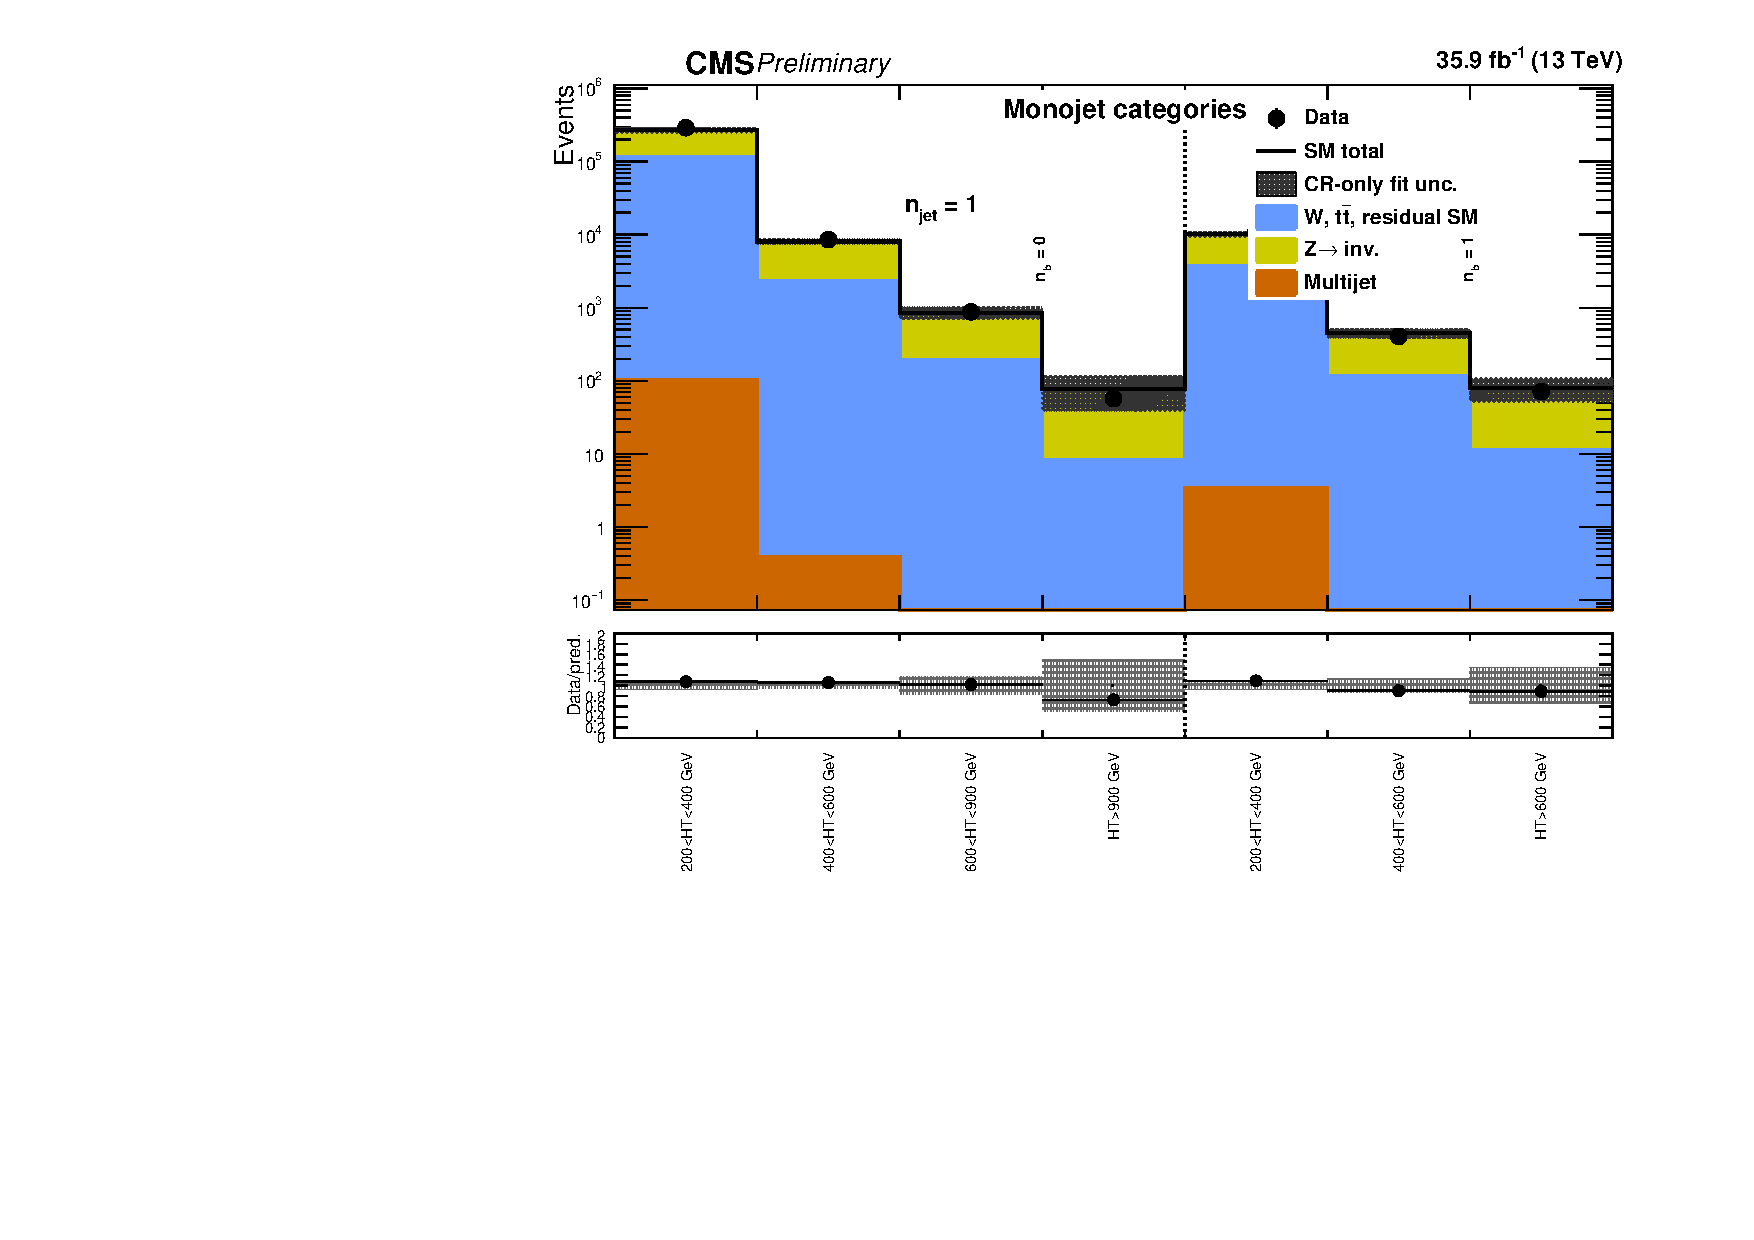
\includegraphics[width=1.\linewidth]{figures/results/36invfb/mono/summaryPlot_Monojet_prefit}
\end{figure}

\clearpage
\begin{figure}[h!]
  \centering
  \caption{Upper panel. Event yields observed in data (solid circles)
    and SM expectations with their associated uncertainties (black
    histogram with shaded band) as a function of \nb and \scalht,
    integrated over \mht, and for the monojet category ($\njet = 1$)
    in the signal region. Lower panel. Data-to-background ratios. The
    background estimates and ratios are obtained with the full fit. }
  \label{fig:mr_mono_post}
  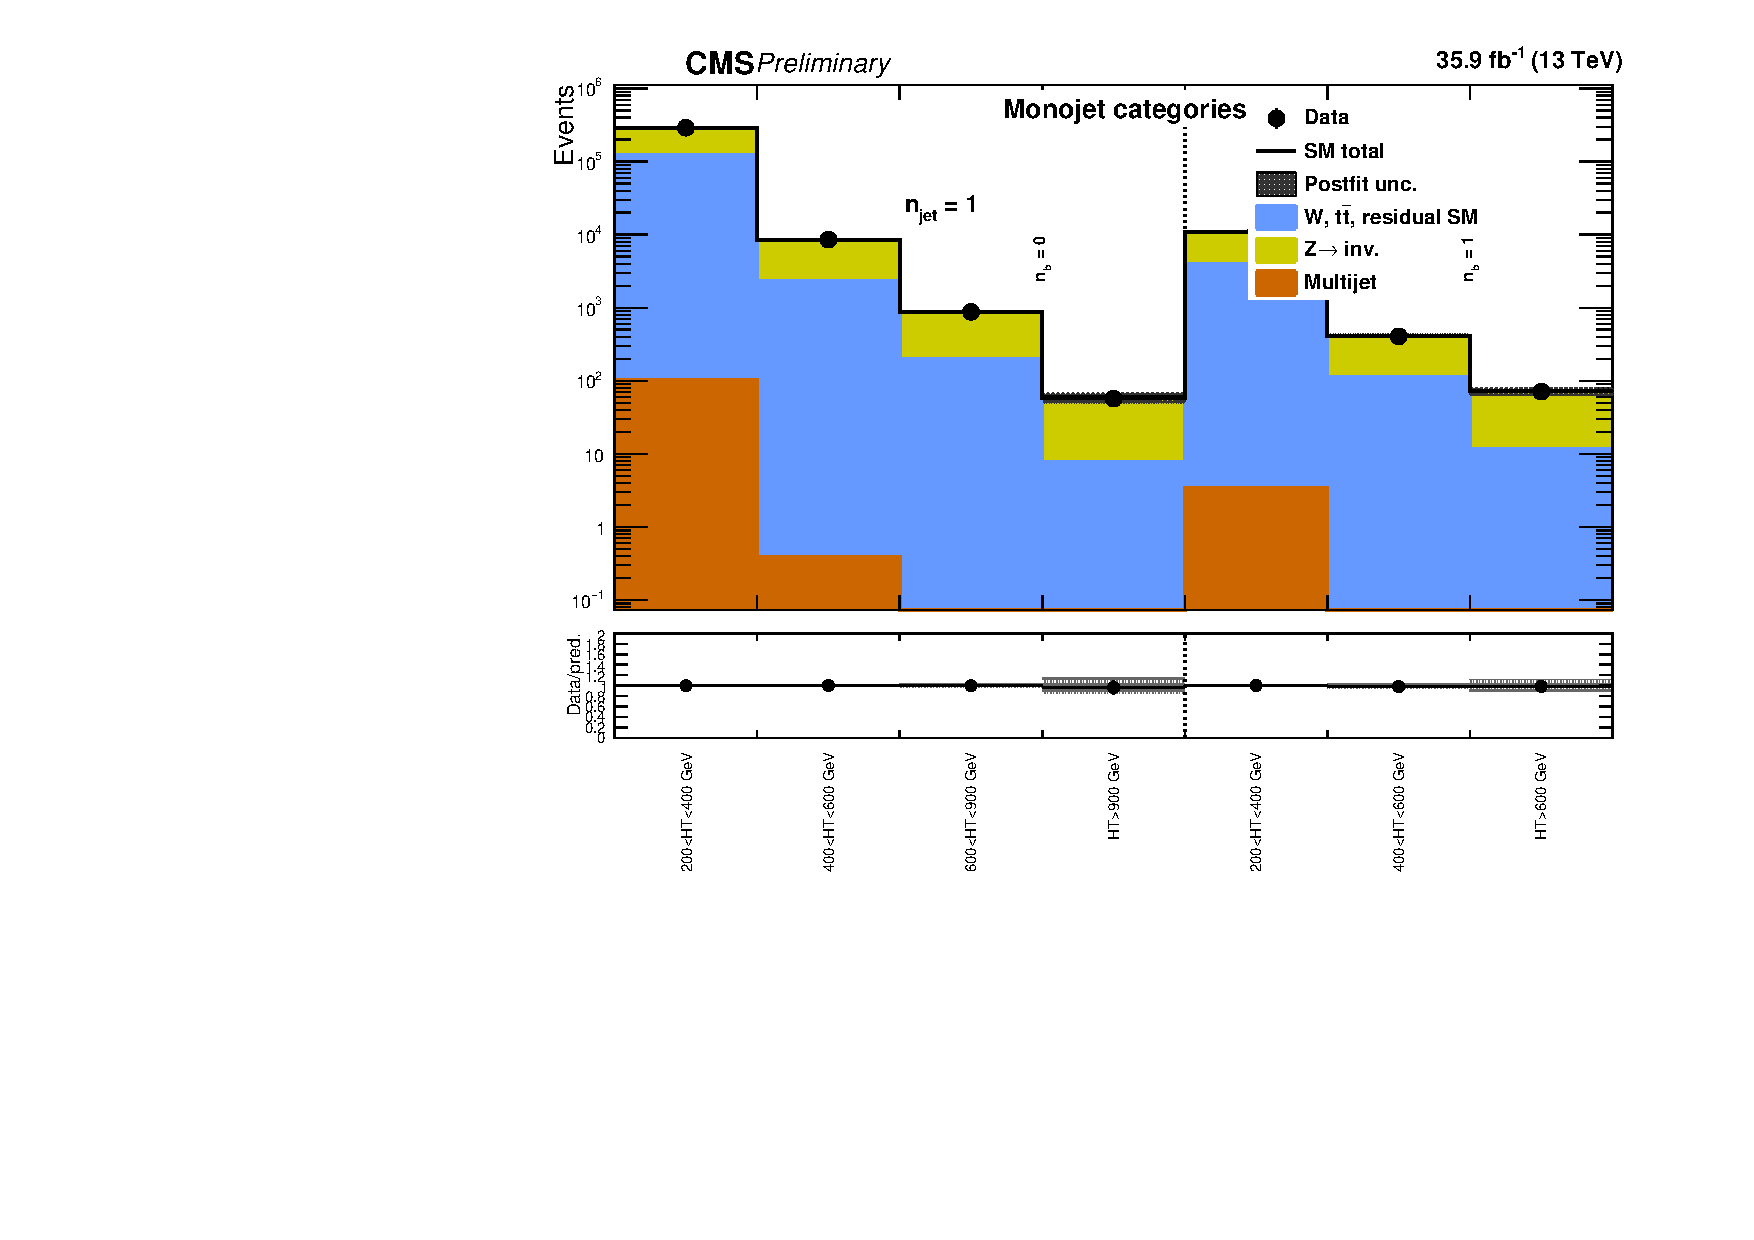
\includegraphics[width=1.\linewidth]{figures/results/36invfb/mono/summaryPlot_Monojet_fit_b}
\end{figure}

\clearpage
\begin{figure}[h!]
  \centering
  \caption{Upper panel. Event yields observed in data (solid circles)
    and SM expectations with their associated uncertainties (black
    histogram with shaded band) as a function of \nb and \scalht,
    integrated over \mht, and for the monojet category ($\njet = 1$)
    in the signal region. Lower panel. The pulls, which are obtained
    from both the masked (red markers) and full (blue markers) fits. }
  \label{fig:mr_mono_pulls}
  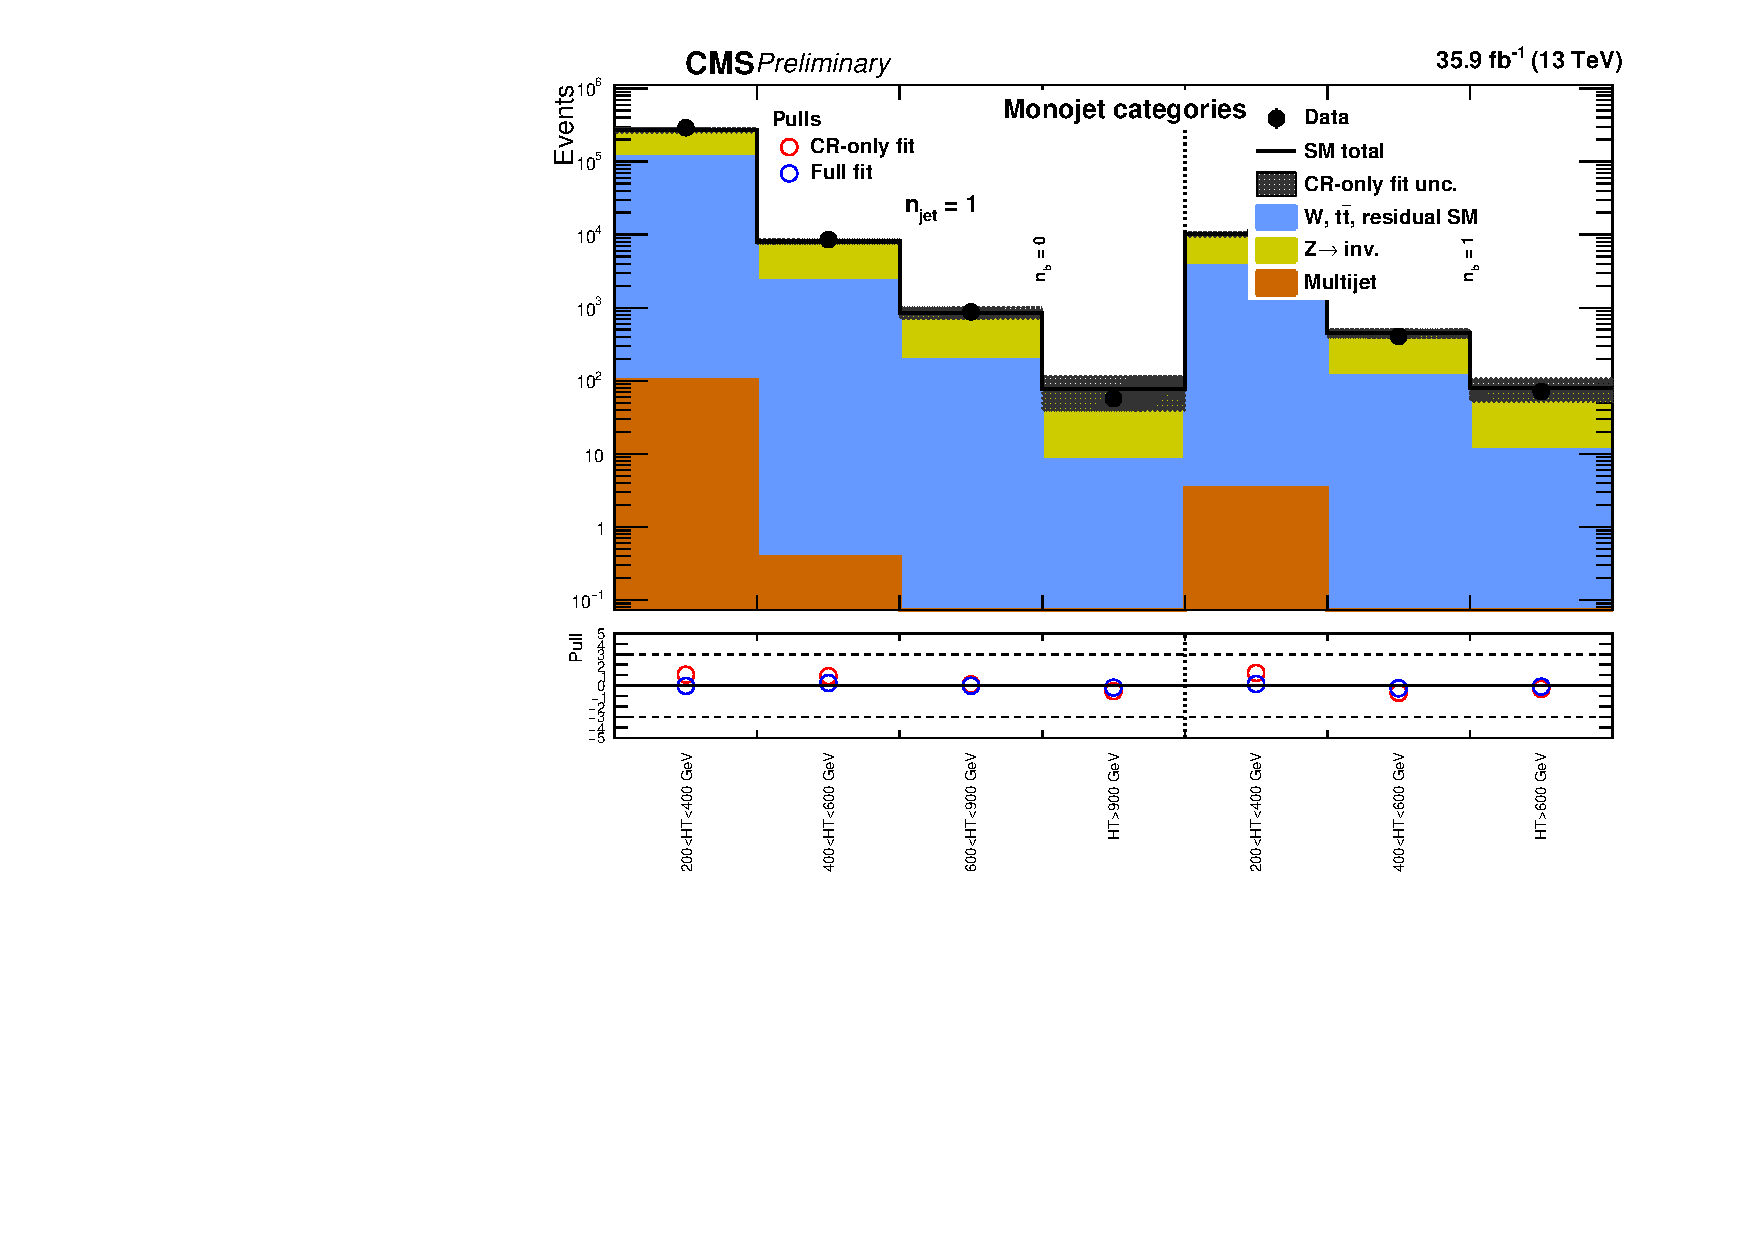
\includegraphics[width=1.\linewidth]{figures/results/36invfb/mono/summaryPlot_Monojet_prefit_overlay_fit_b}
\end{figure}

% asym 
\clearpage
\subsection{Asymmetric topology}

\begin{figure}[h!]
  \centering
  \caption{Upper panel. Event yields observed in data (solid circles)
    and SM expectations with their associated uncertainties (black
    histogram with shaded band) as a function of \nb and \scalht,
    integrated over \mht, and for the asymmetric \njet category
    in the signal region. Lower panel. Data-to-background ratios. The
    background estimates and ratios are from the masked fit. }
  \label{fig:mr_asym_pre}
  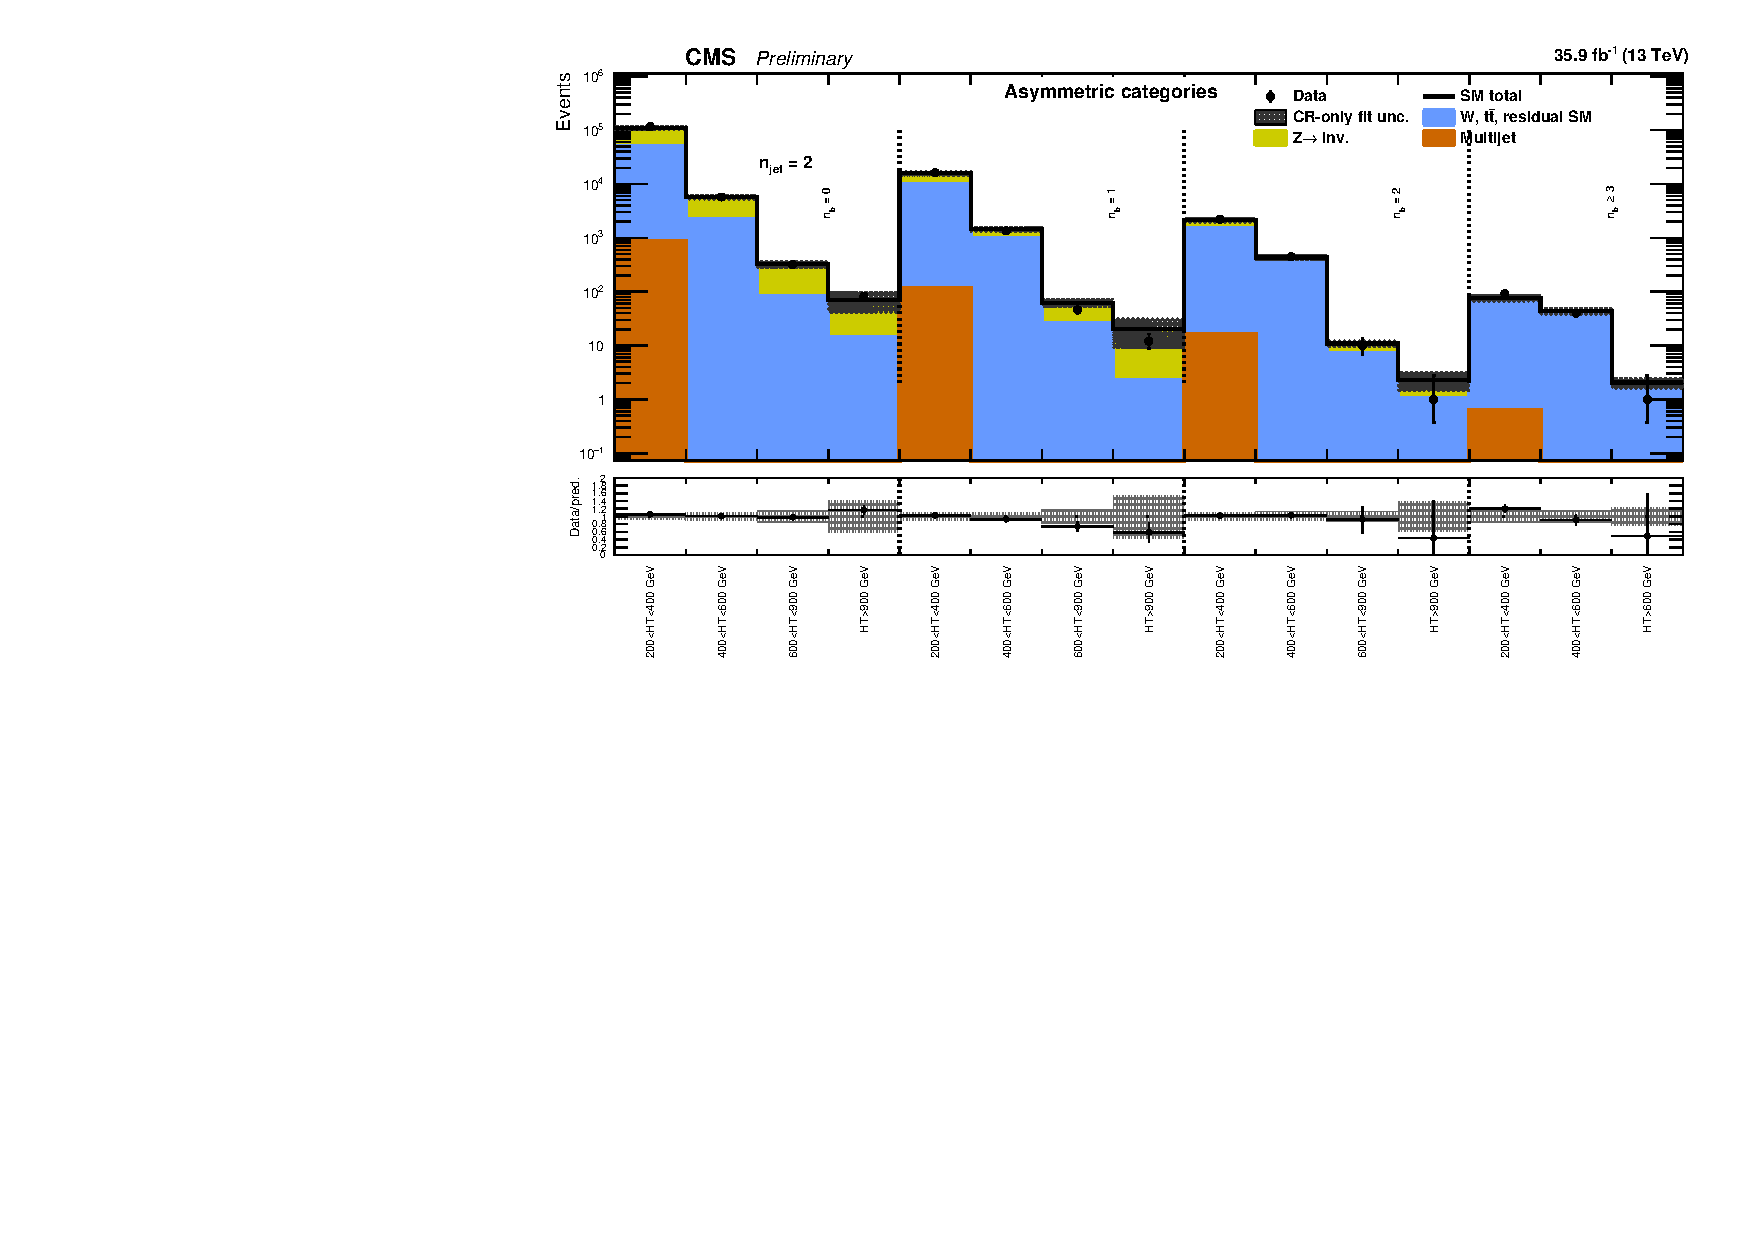
\includegraphics[width=1.\linewidth]{figures/results/36invfb/asym/summaryPlot_Asymmetric_prefit}
\end{figure}

\clearpage
\begin{figure}[h!]
  \centering
  \caption{Upper panel. Event yields observed in data (solid circles)
    and SM expectations with their associated uncertainties (black
    histogram with shaded band) as a function of \nb and \scalht,
    integrated over \mht, and for the asymmetric \njet category
    in the signal region. Lower panel. Data-to-background ratios. The
    background estimates and ratios are obtained with the full fit. }
  \label{fig:mr_asym_post}
  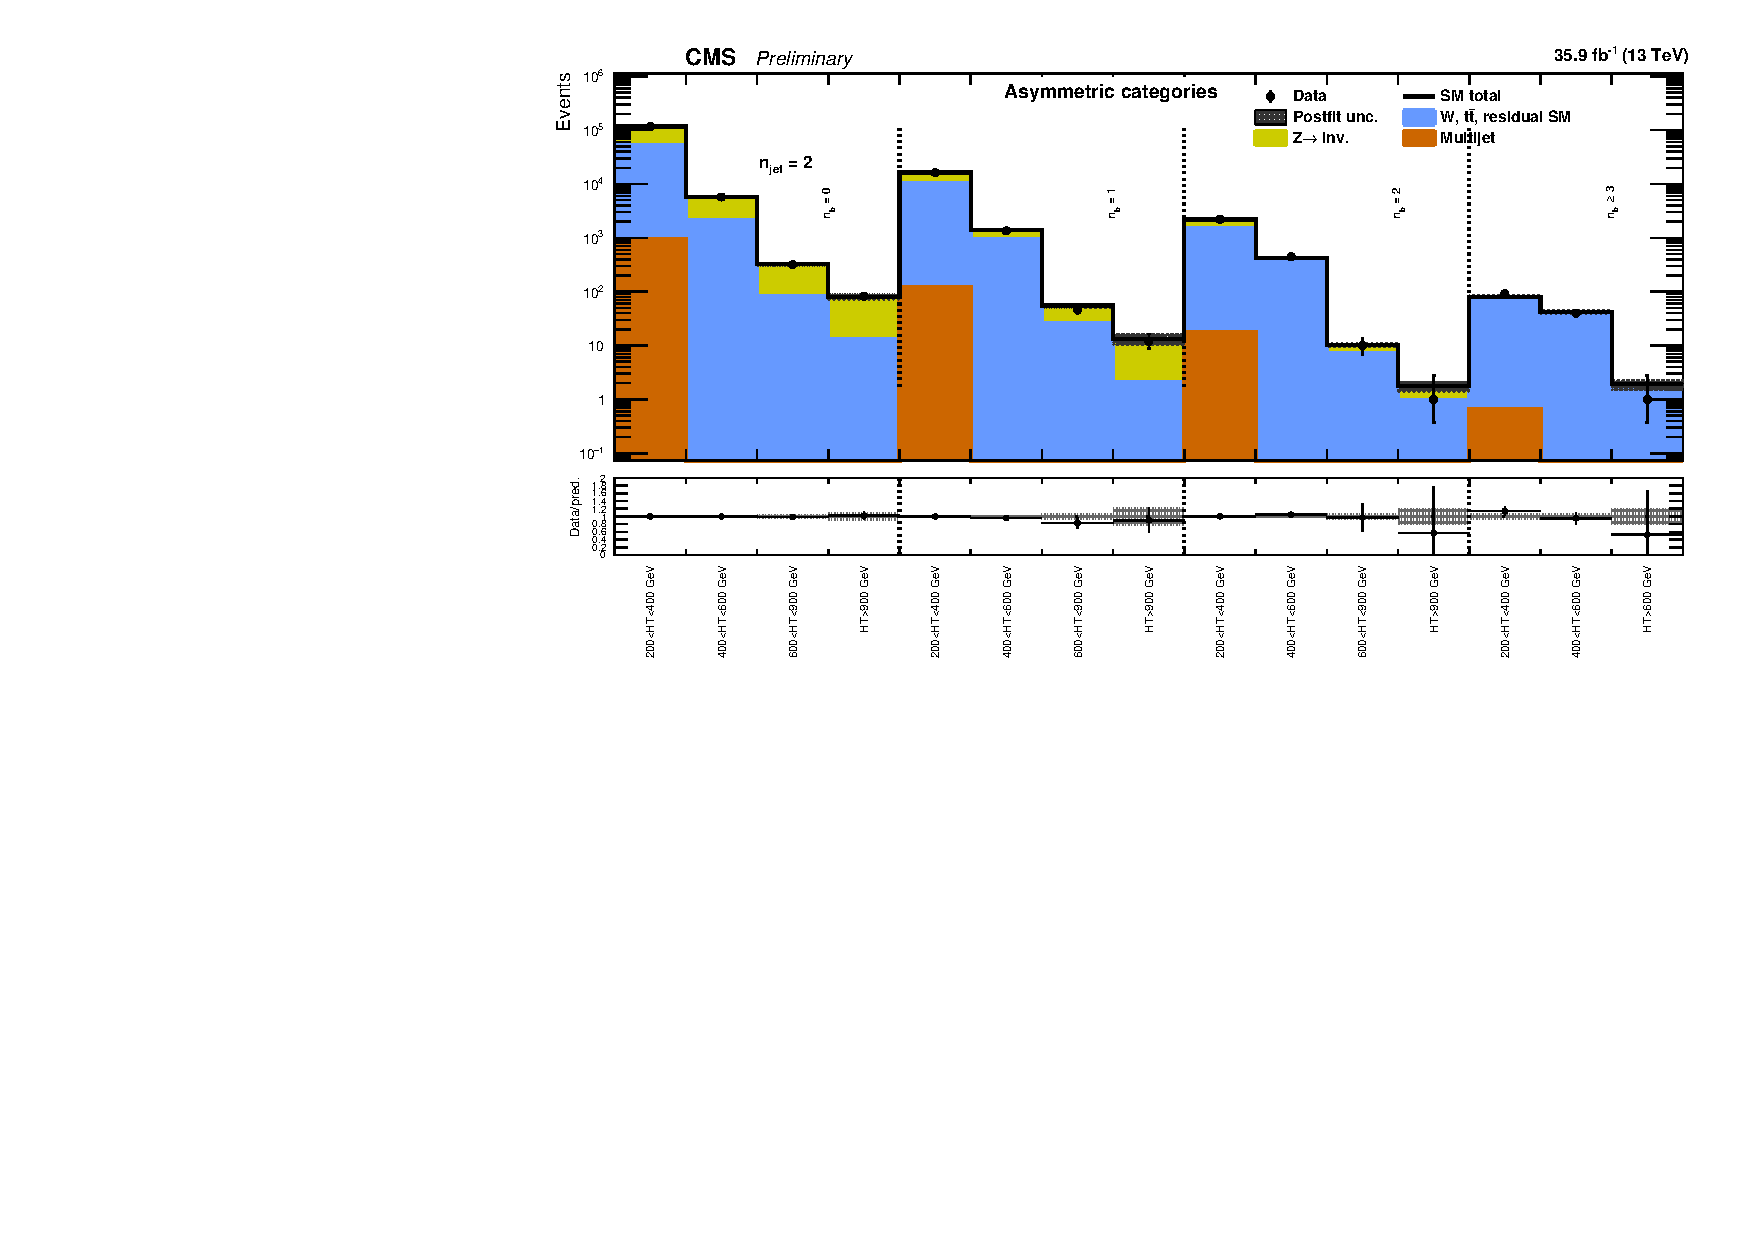
\includegraphics[width=1.\linewidth]{figures/results/36invfb/asym/summaryPlot_Asymmetric_fit_b}
\end{figure}

\clearpage
\begin{figure}[h!]
  \centering
  \caption{Upper panel. Event yields observed in data (solid circles)
    and SM expectations with their associated uncertainties (black
    histogram with shaded band) as a function of \nb and \scalht,
    integrated over \mht, and for the asymmetric \njet category
    in the signal region. Lower panel. The pulls, which are obtained
    from both the masked (red markers) and full (blue markers) fits. }
  \label{fig:mr_asym_pulls}
  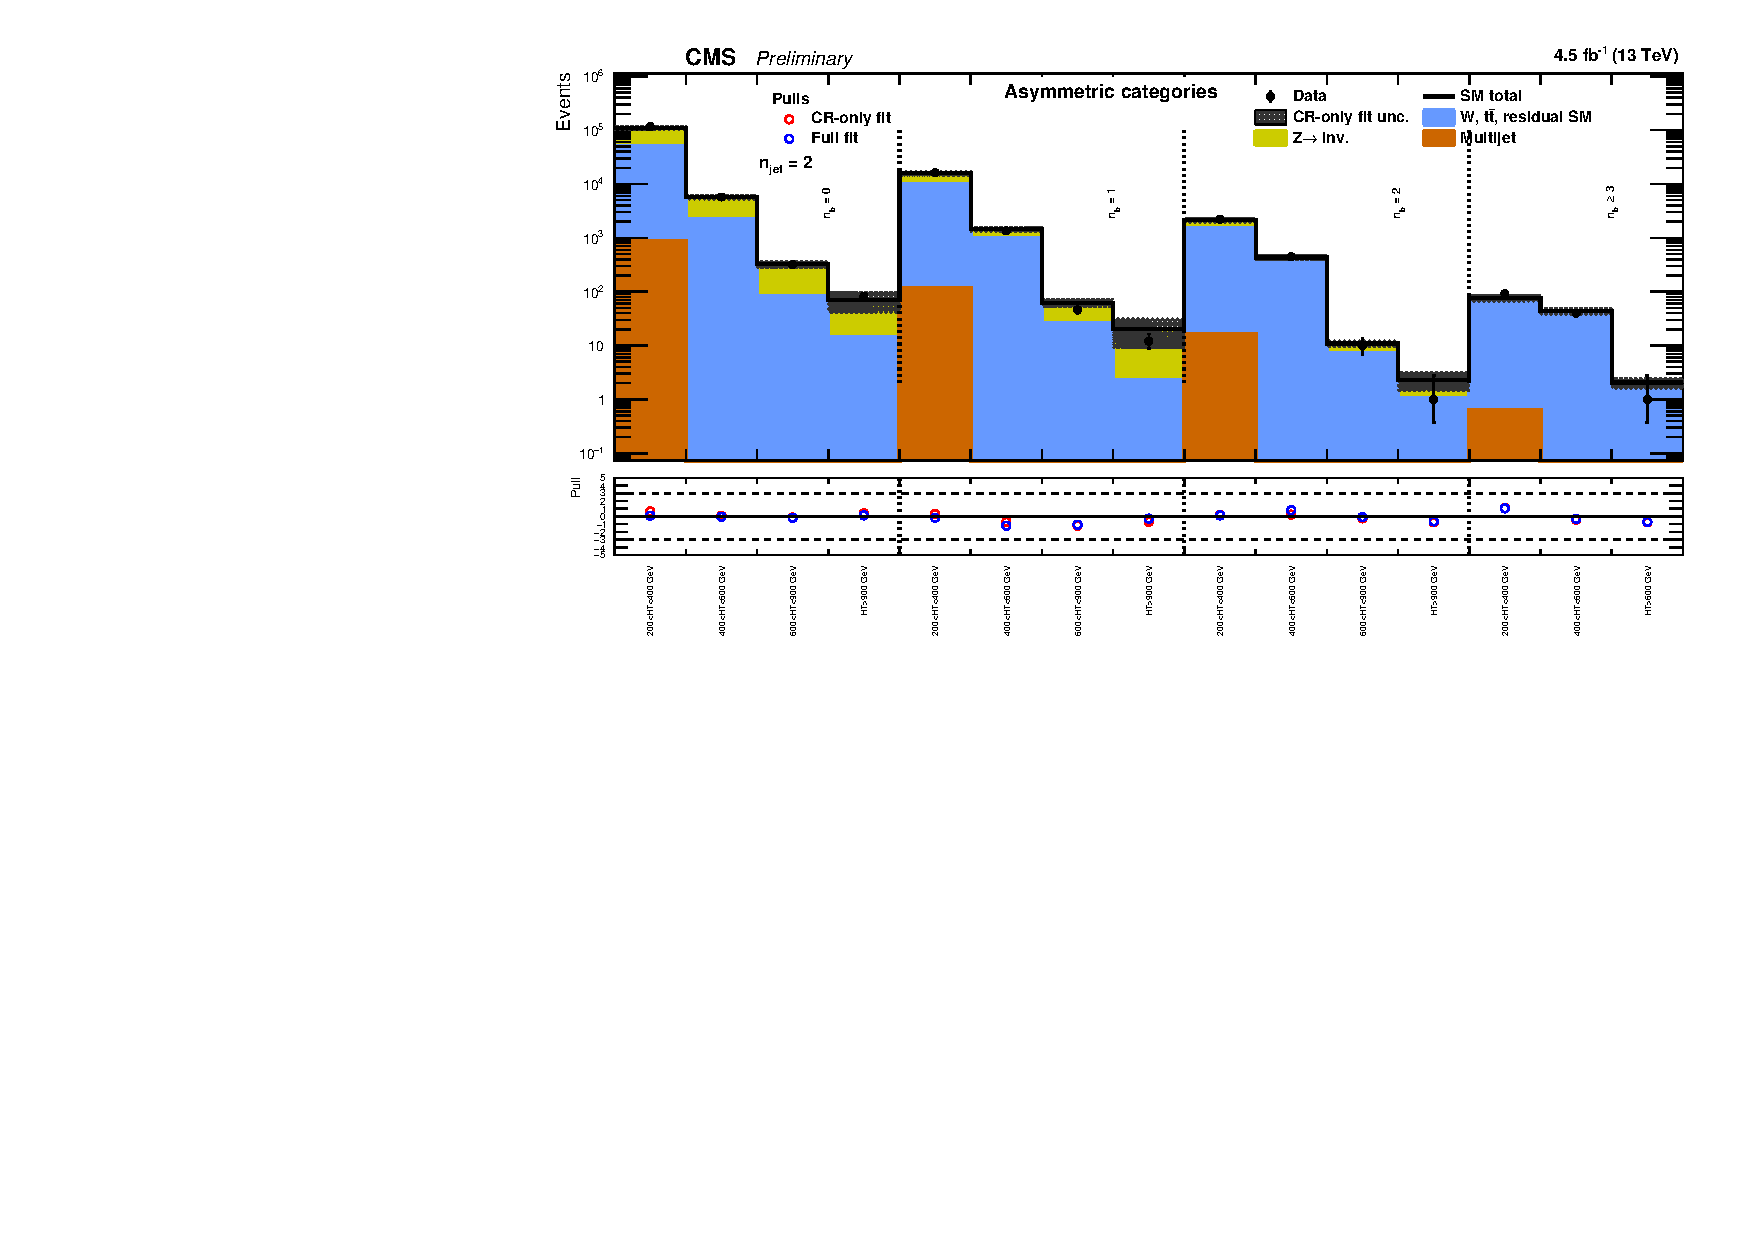
\includegraphics[width=1.\linewidth]{figures/results/36invfb/asym/summaryPlot_Asymmetric_prefit_overlay_fit_b}
\end{figure}

% symm
\clearpage
\subsection{Symmetric topology}

\begin{figure}[h!]
  \centering
  \caption{Upper panel. Event yields observed in data (solid circles)
    and SM expectations with their associated uncertainties (black
    histogram with shaded band) as a function of \nb and \scalht,
    integrated over \mht, and for the symmmetric \njet category
    in the signal region. Lower panel. Data-to-background ratios. The
    background estimates and ratios are from the masked fit. }
  \label{fig:mr_symm_pre}
  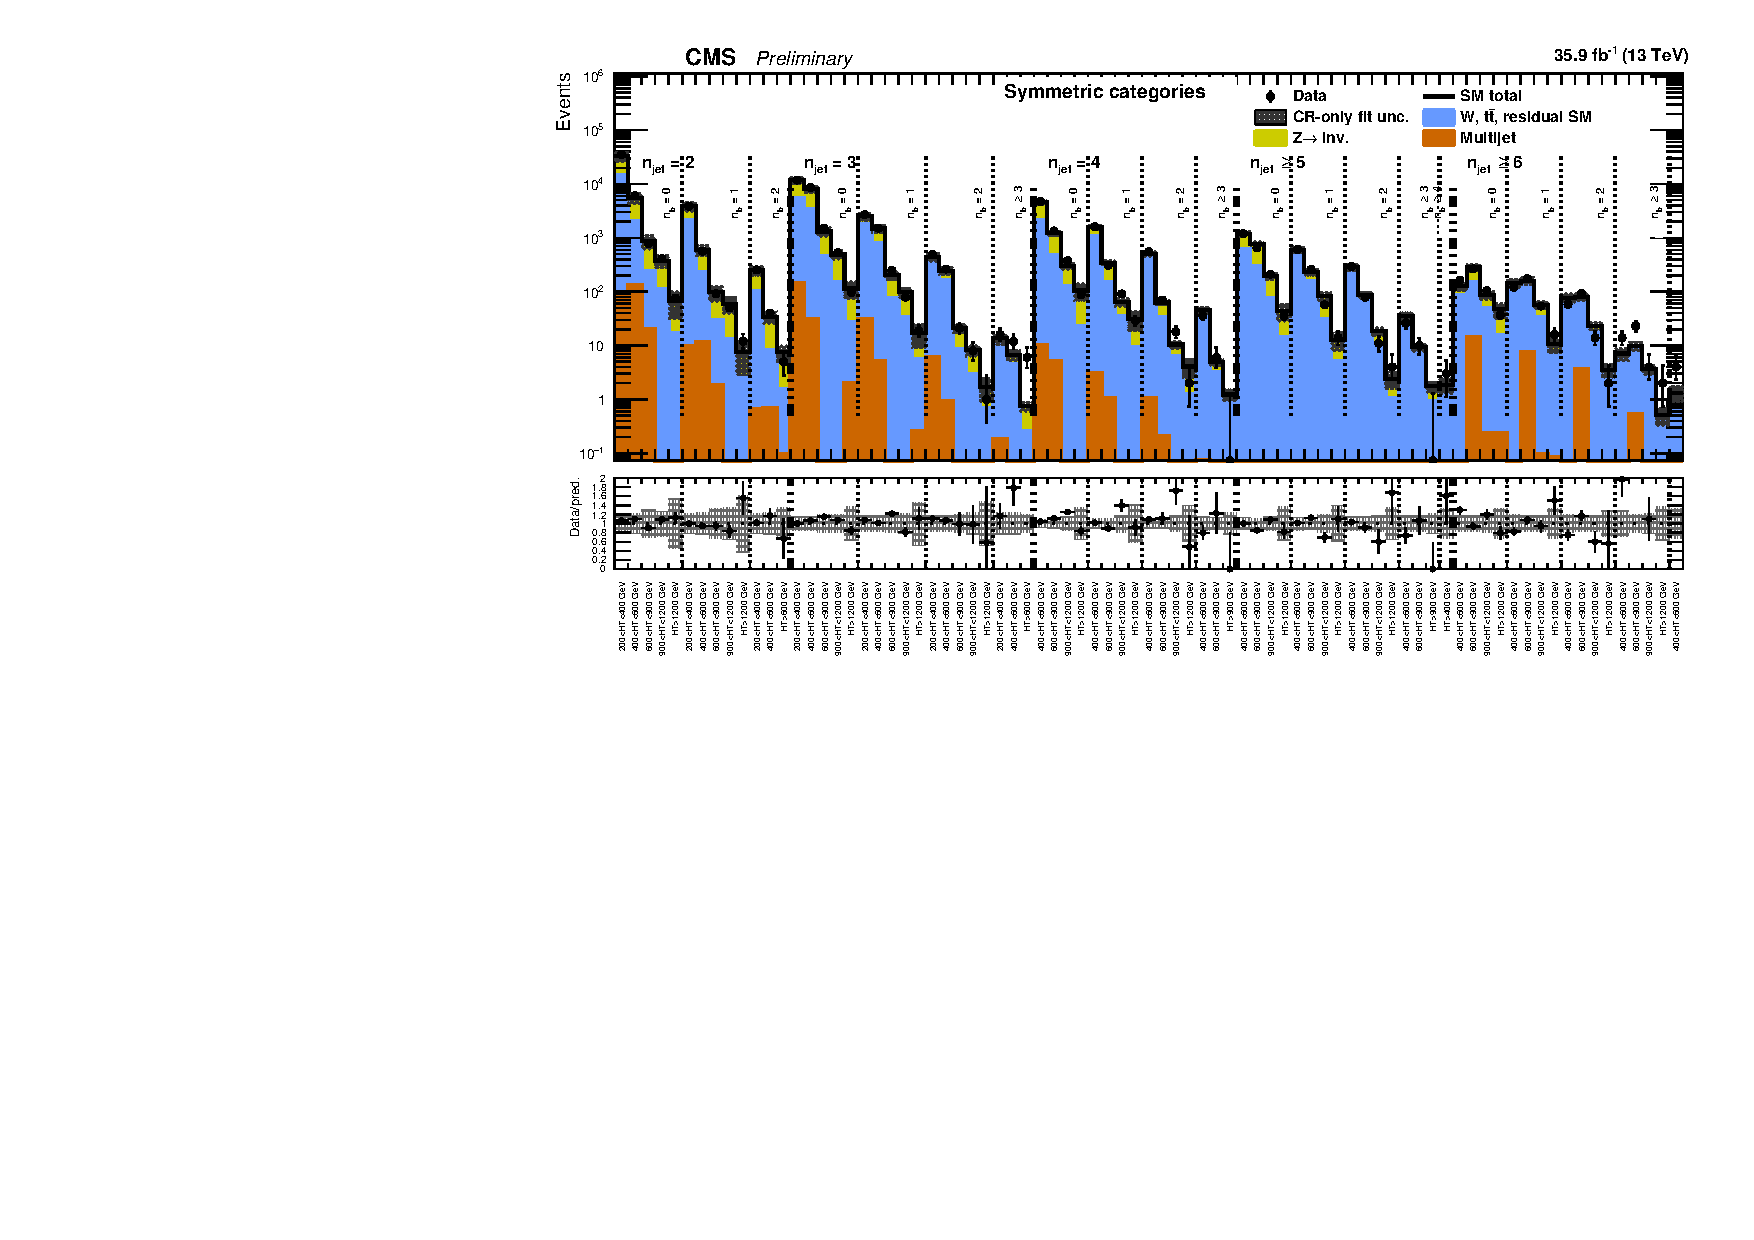
\includegraphics[width=1.\linewidth]{figures/results/36invfb/symm/summaryPlot_Symmetric_prefit}
\end{figure}

\clearpage
\begin{figure}[h!]
  \centering
  \caption{Upper panel. Event yields observed in data (solid circles)
    and SM expectations with their associated uncertainties (black
    histogram with shaded band) as a function of \nb and \scalht,
    integrated over \mht, and for the symmmetric \njet category
    in the signal region. Lower panel. Data-to-background ratios. The
    background estimates and ratios are obtained with the full fit. }
  \label{fig:mr_symm_post}
  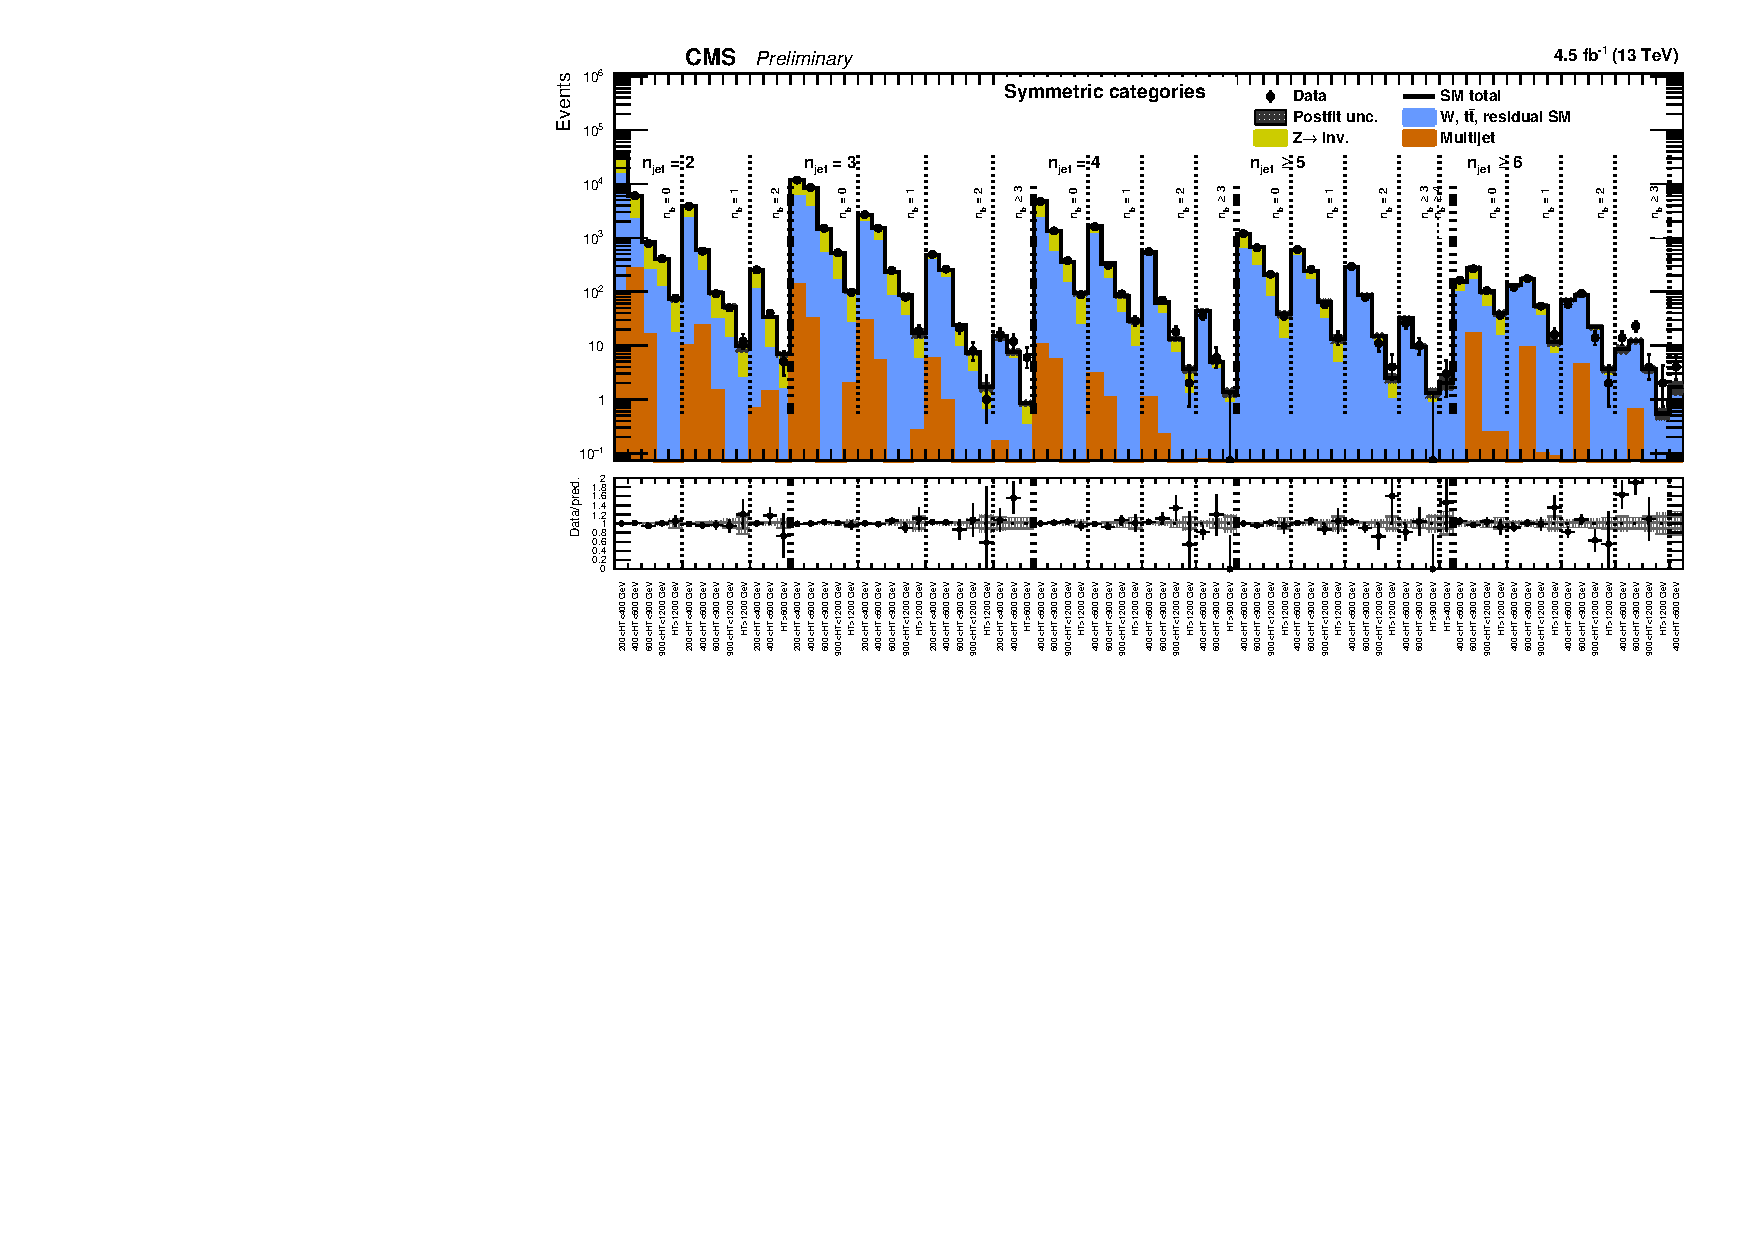
\includegraphics[width=1.\linewidth]{figures/results/36invfb/symm/summaryPlot_Symmetric_fit_b}
\end{figure}

\clearpage
\begin{figure}[h!]
  \centering
  \caption{Upper panel. Event yields observed in data (solid circles)
    and SM expectations with their associated uncertainties (black
    histogram with shaded band) as a function of \nb and \scalht,
    integrated over \mht, and for the symmmetric \njet category
    in the signal region. Lower panel. The pulls, which are obtained
    from both the masked (red markers) and full (blue markers) fits. }
  \label{fig:mr_symm_pulls}
  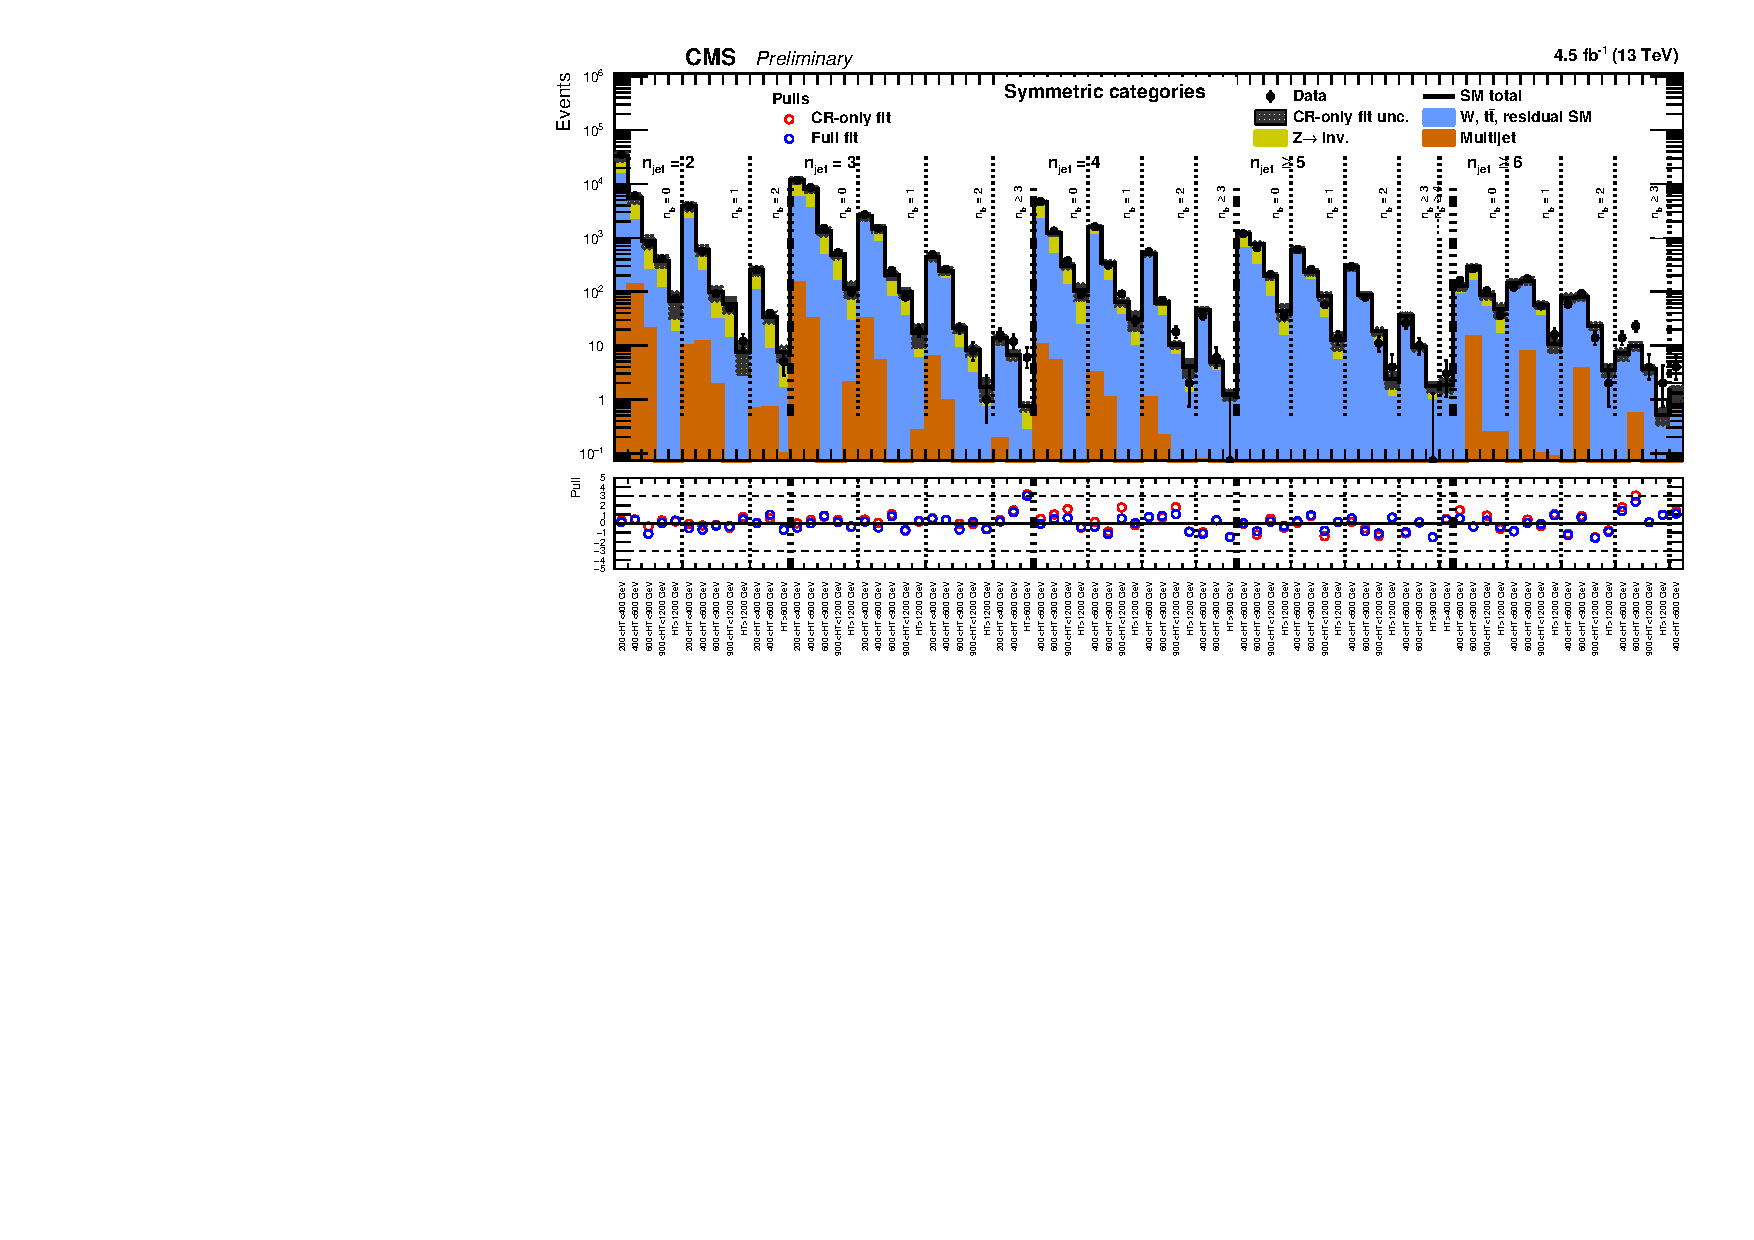
\includegraphics[width=1.\linewidth]{figures/results/36invfb/symm/summaryPlot_Symmetric_prefit_overlay_fit_b}
\end{figure}

% 1d histograms 
\clearpage
\subsection{Ratios and pulls}

\begin{figure}[h!]
  \centering
  \caption{(Left) Data-to-background ratios for all event categories,
    with counts integrated over \mht, obtained from the masked
    fit. (Right) Pulls for all event categories, with counts
    integrated over \mht, obtained from the masked fit.}
  \label{fig:ratios_and_pulls}
  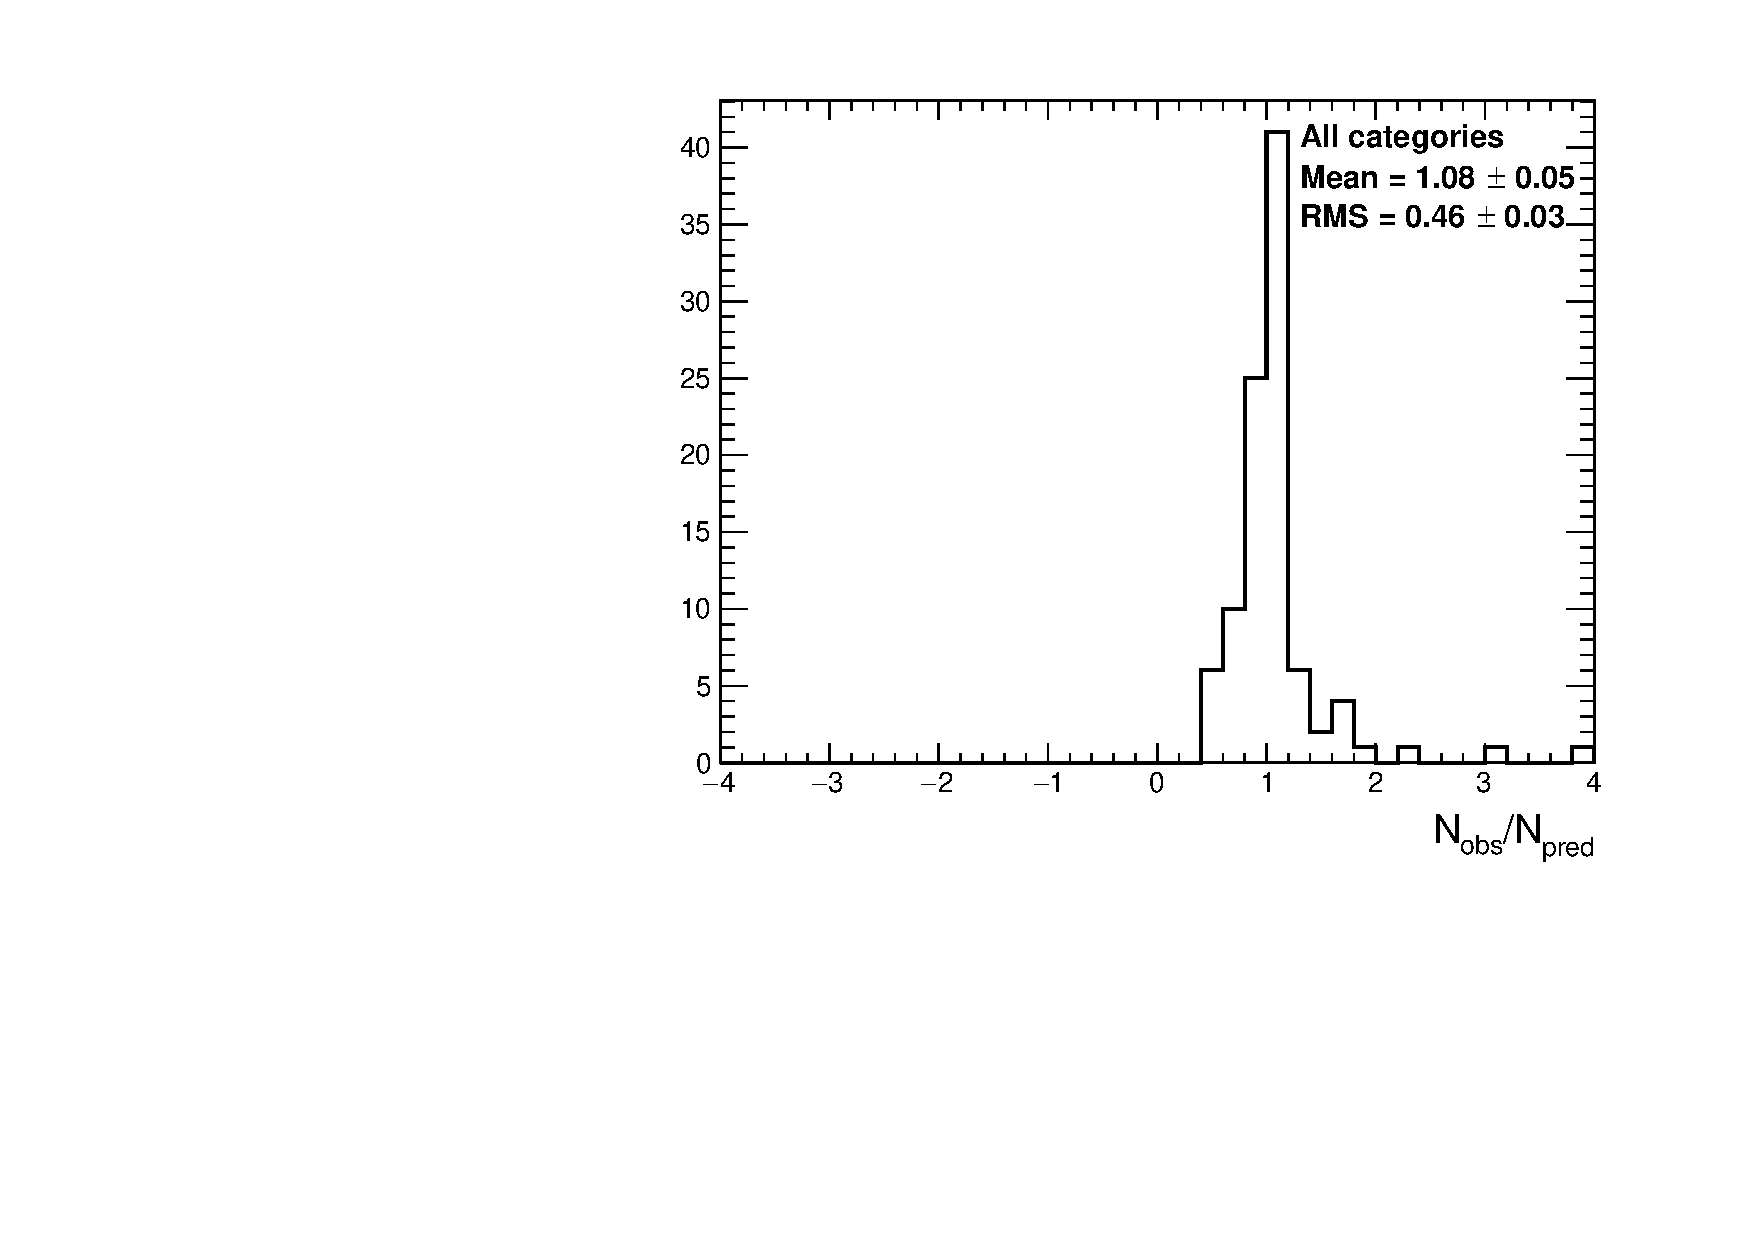
\includegraphics[width=0.49\linewidth]{figures/results/36invfb/all/ratios_all_prefit.pdf}
  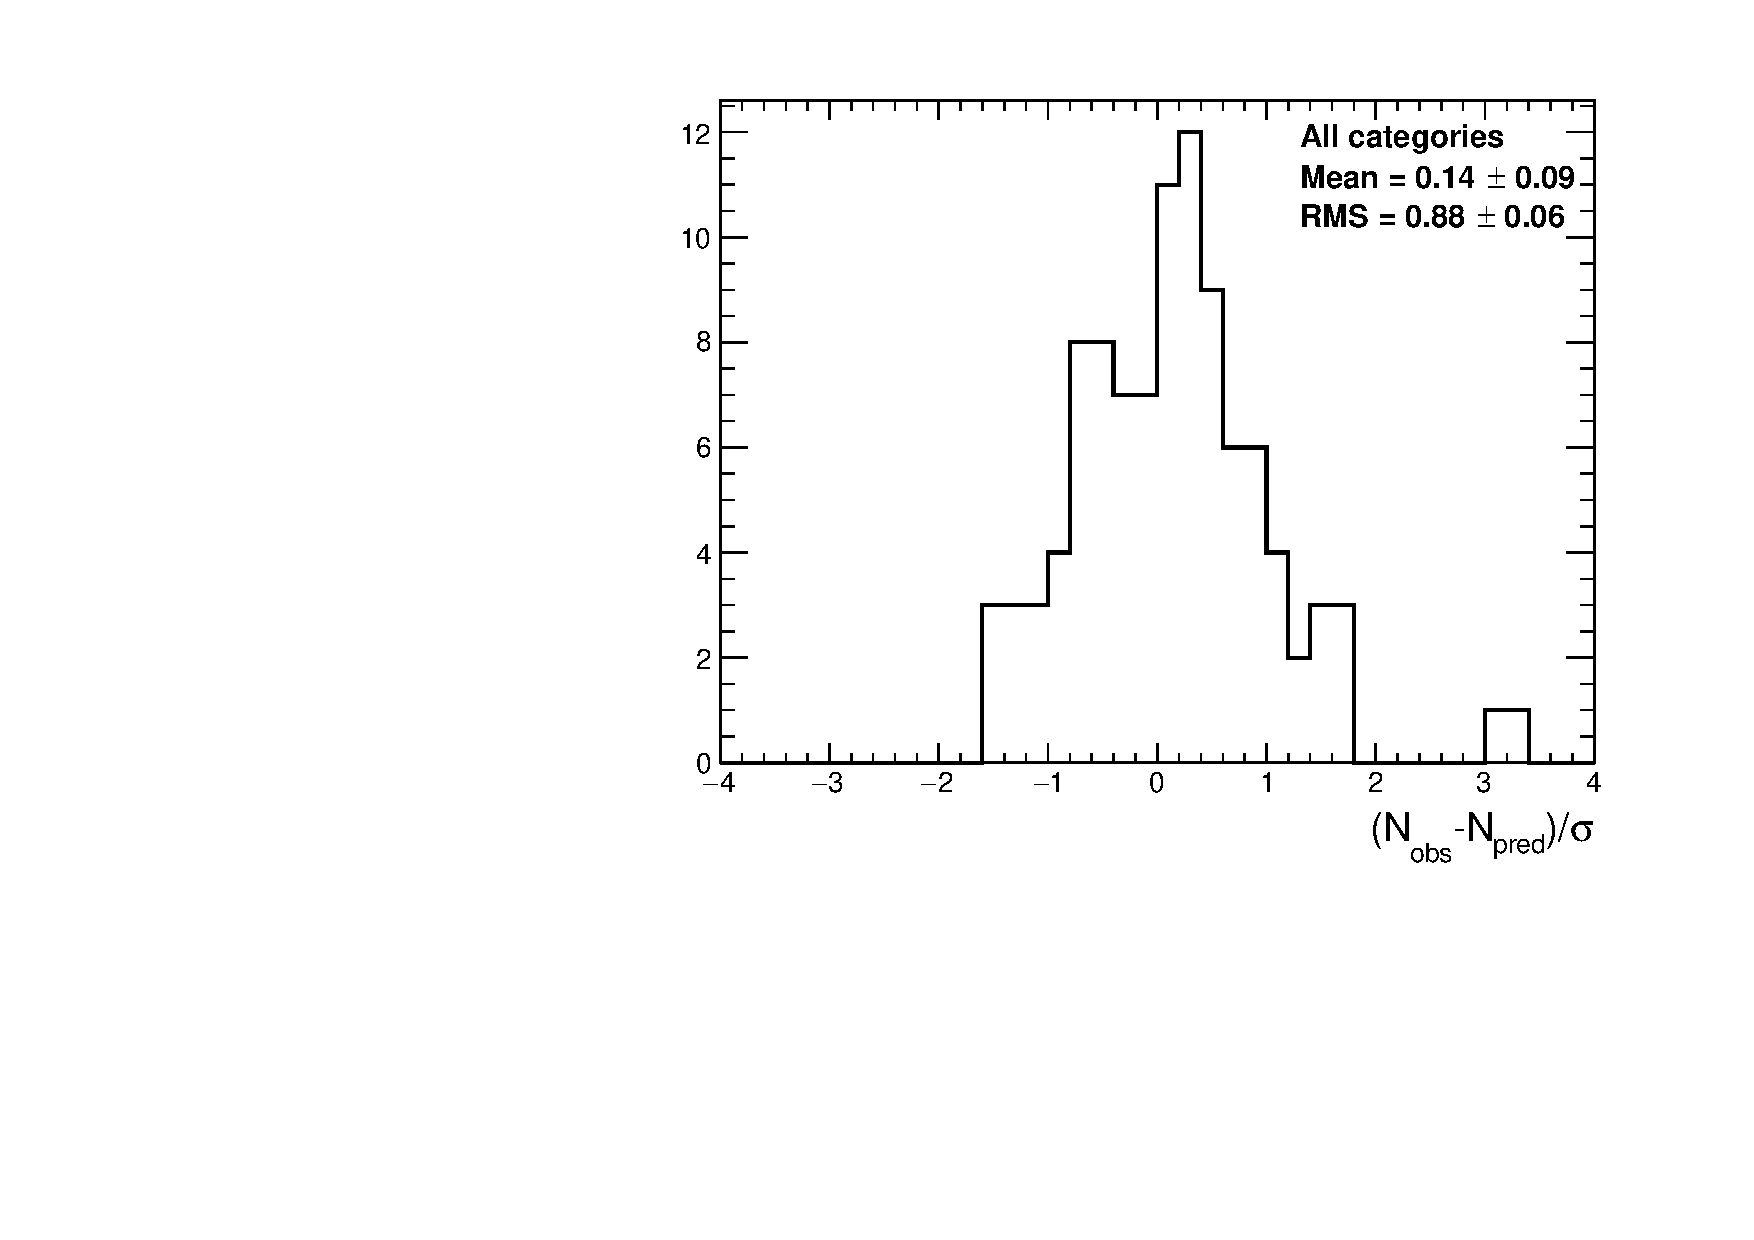
\includegraphics[width=0.49\linewidth]{figures/results/36invfb/all/pulls_all_prefit.pdf}
\end{figure}

\begin{figure}[h!]
  \centering
  \caption{Pulls as a function of (\njet, \nb) event category and
    \scalht [GeV], with counts integrated over \mht, obtained from the
    masked fit.}
  \label{fig:pulls}
  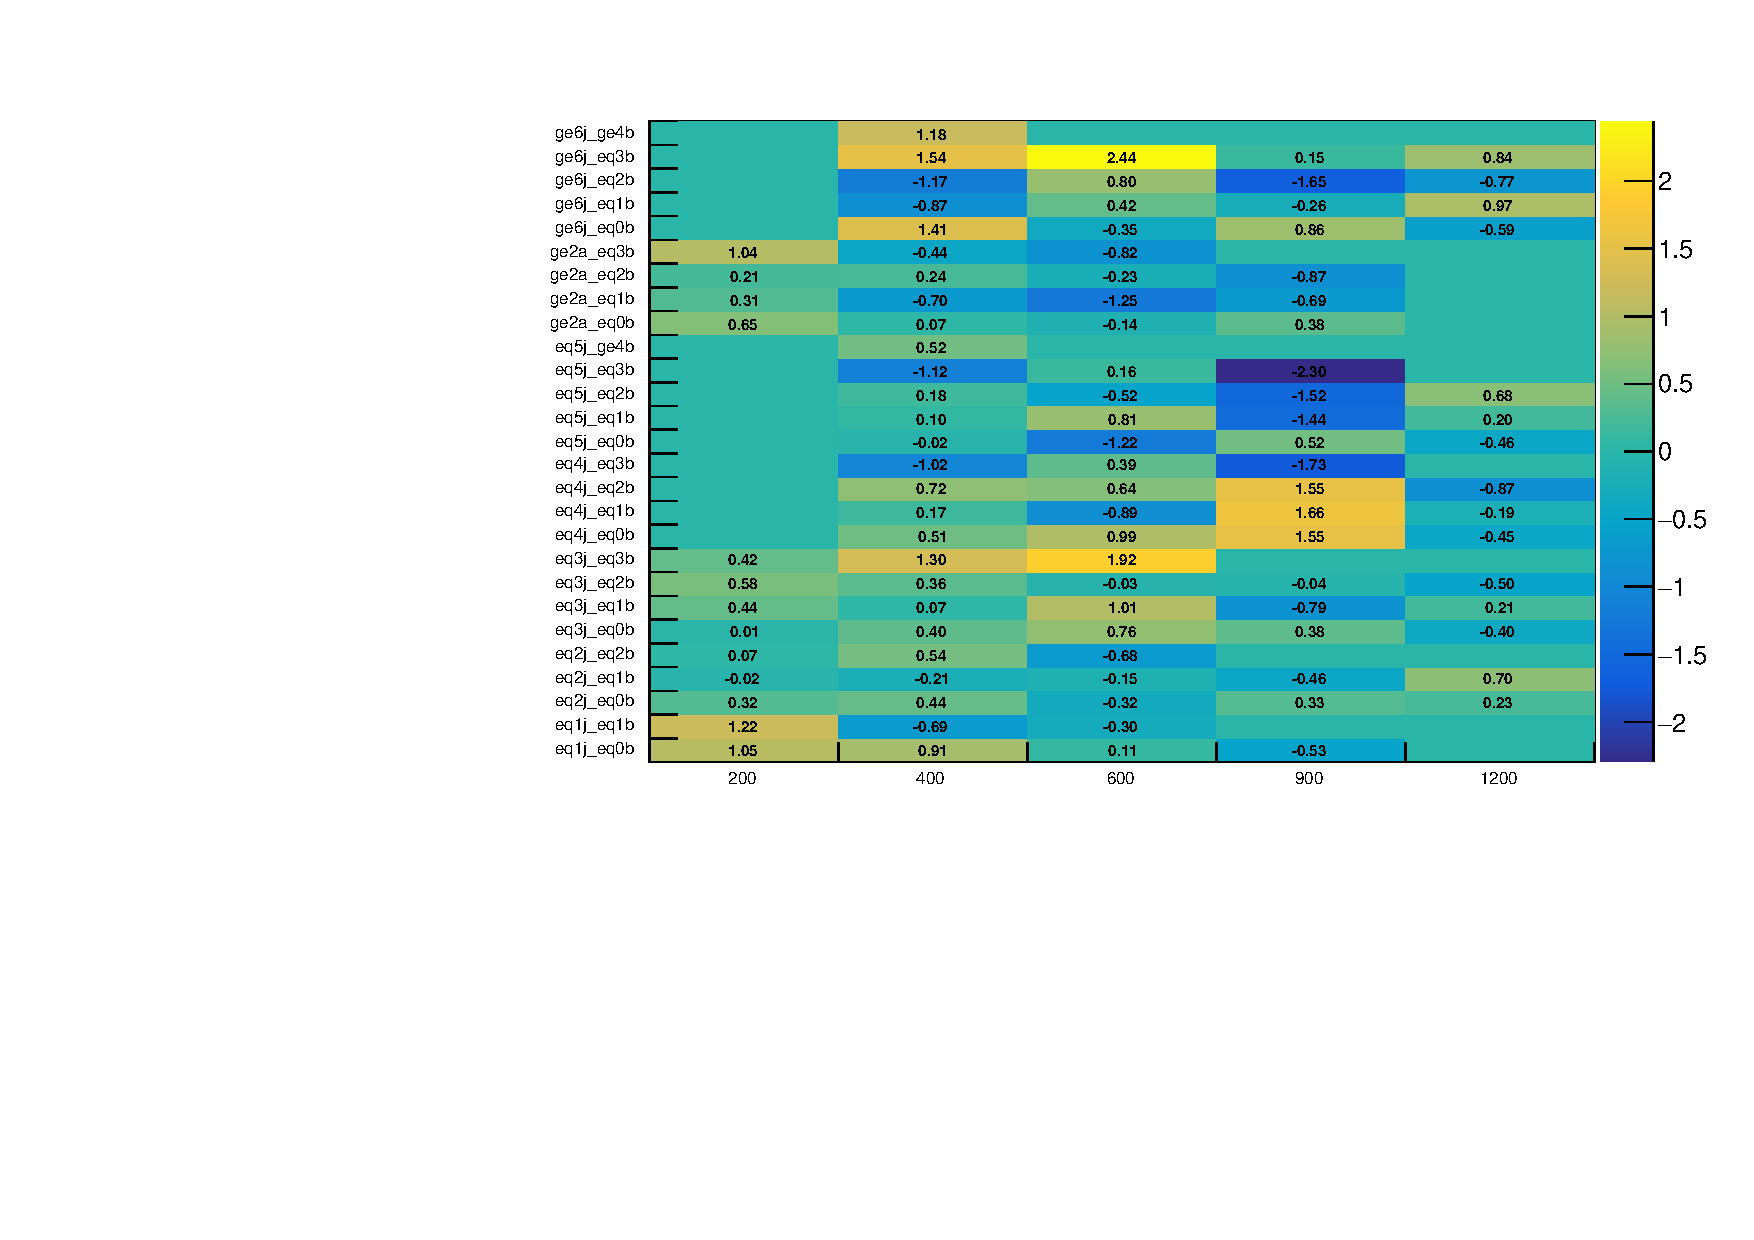
\includegraphics[width=0.8\linewidth]{figures/results/36invfb/all/pull2D_CROnlyFit.pdf}
\end{figure}

\clearpage
\subsection{SM breakdown}

\begin{figure}[h!]
  \centering
  \caption{Breakdown of SM backgrounds in the signal region as
    determined by the CR-only (top) and full (bottom) fits.}
  \label{fig:breakdown}
%  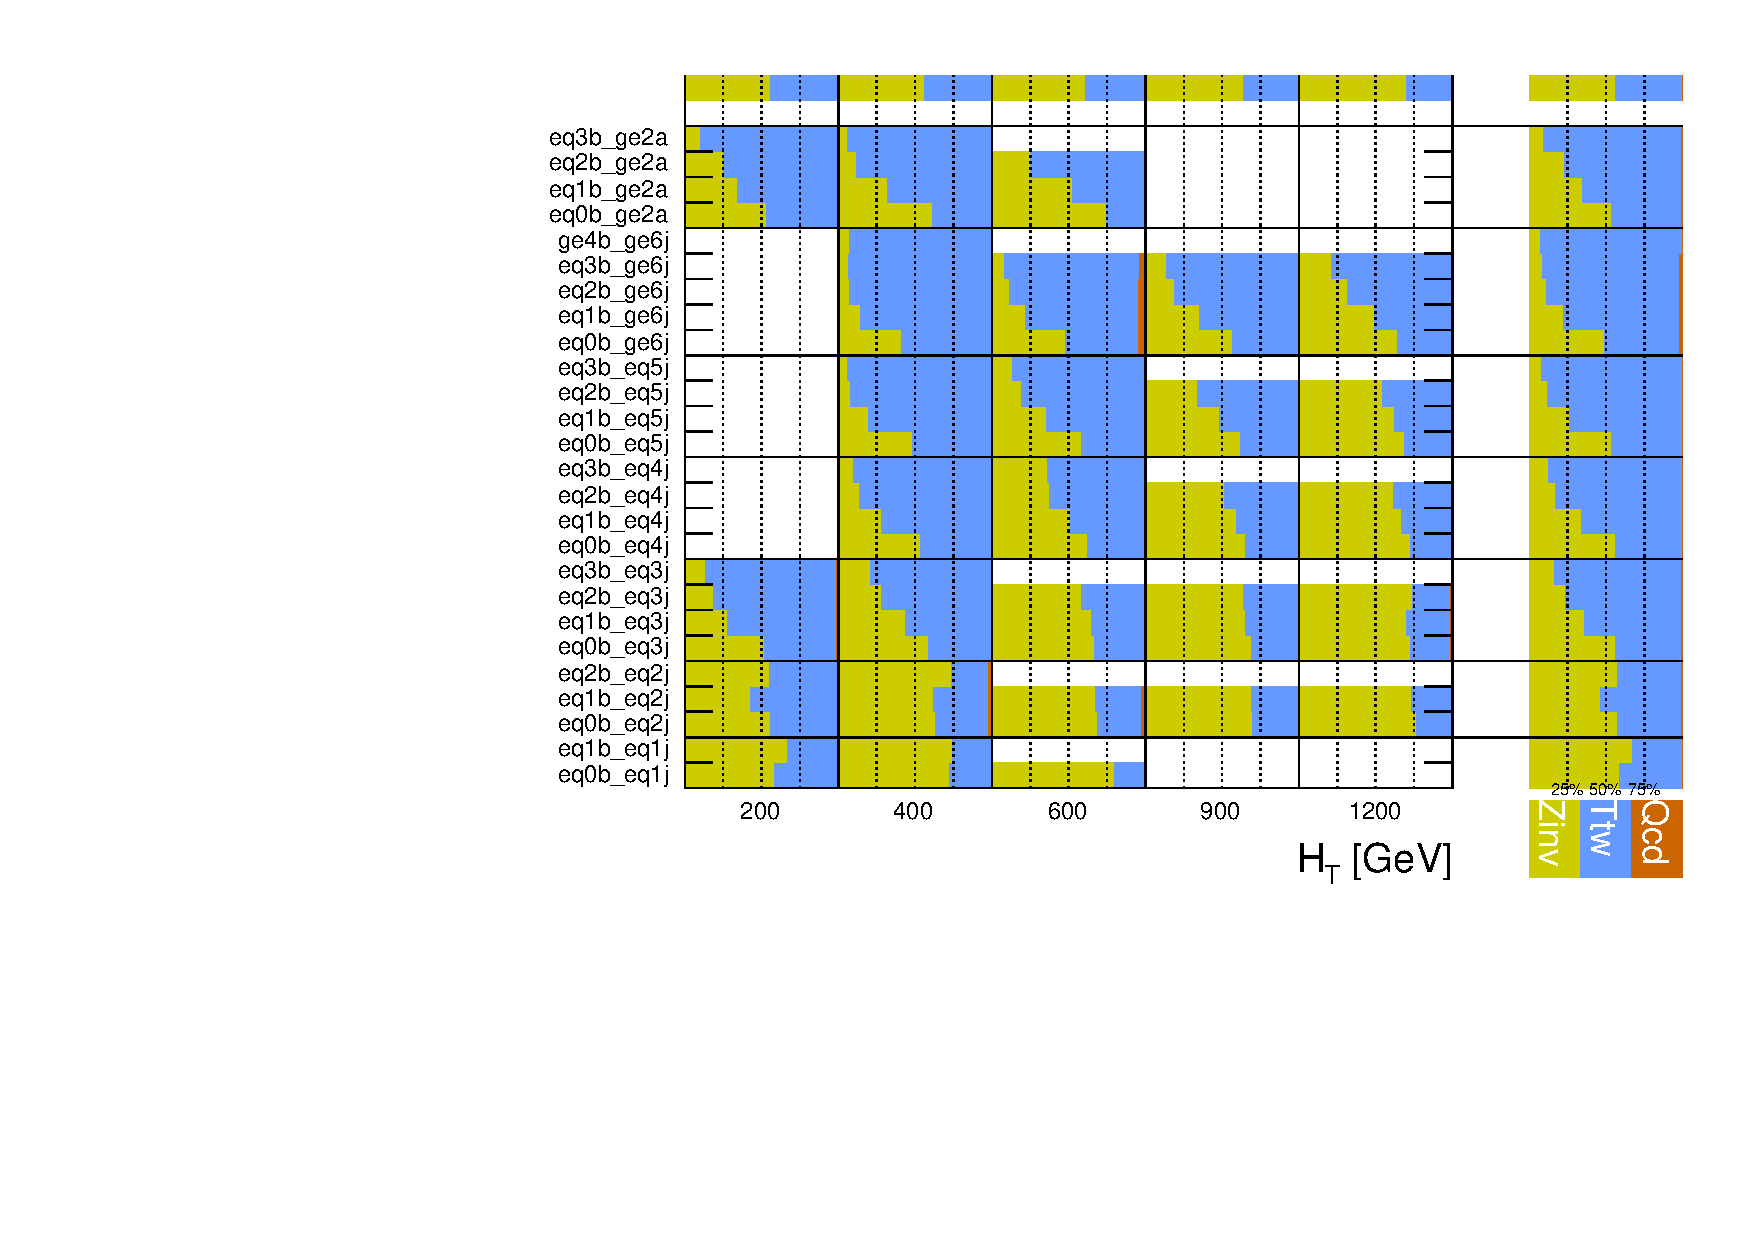
\includegraphics[width=0.6\linewidth]{figures/results/36invfb/breakdown/prefit/Signal_sample_composition.pdf}\\
  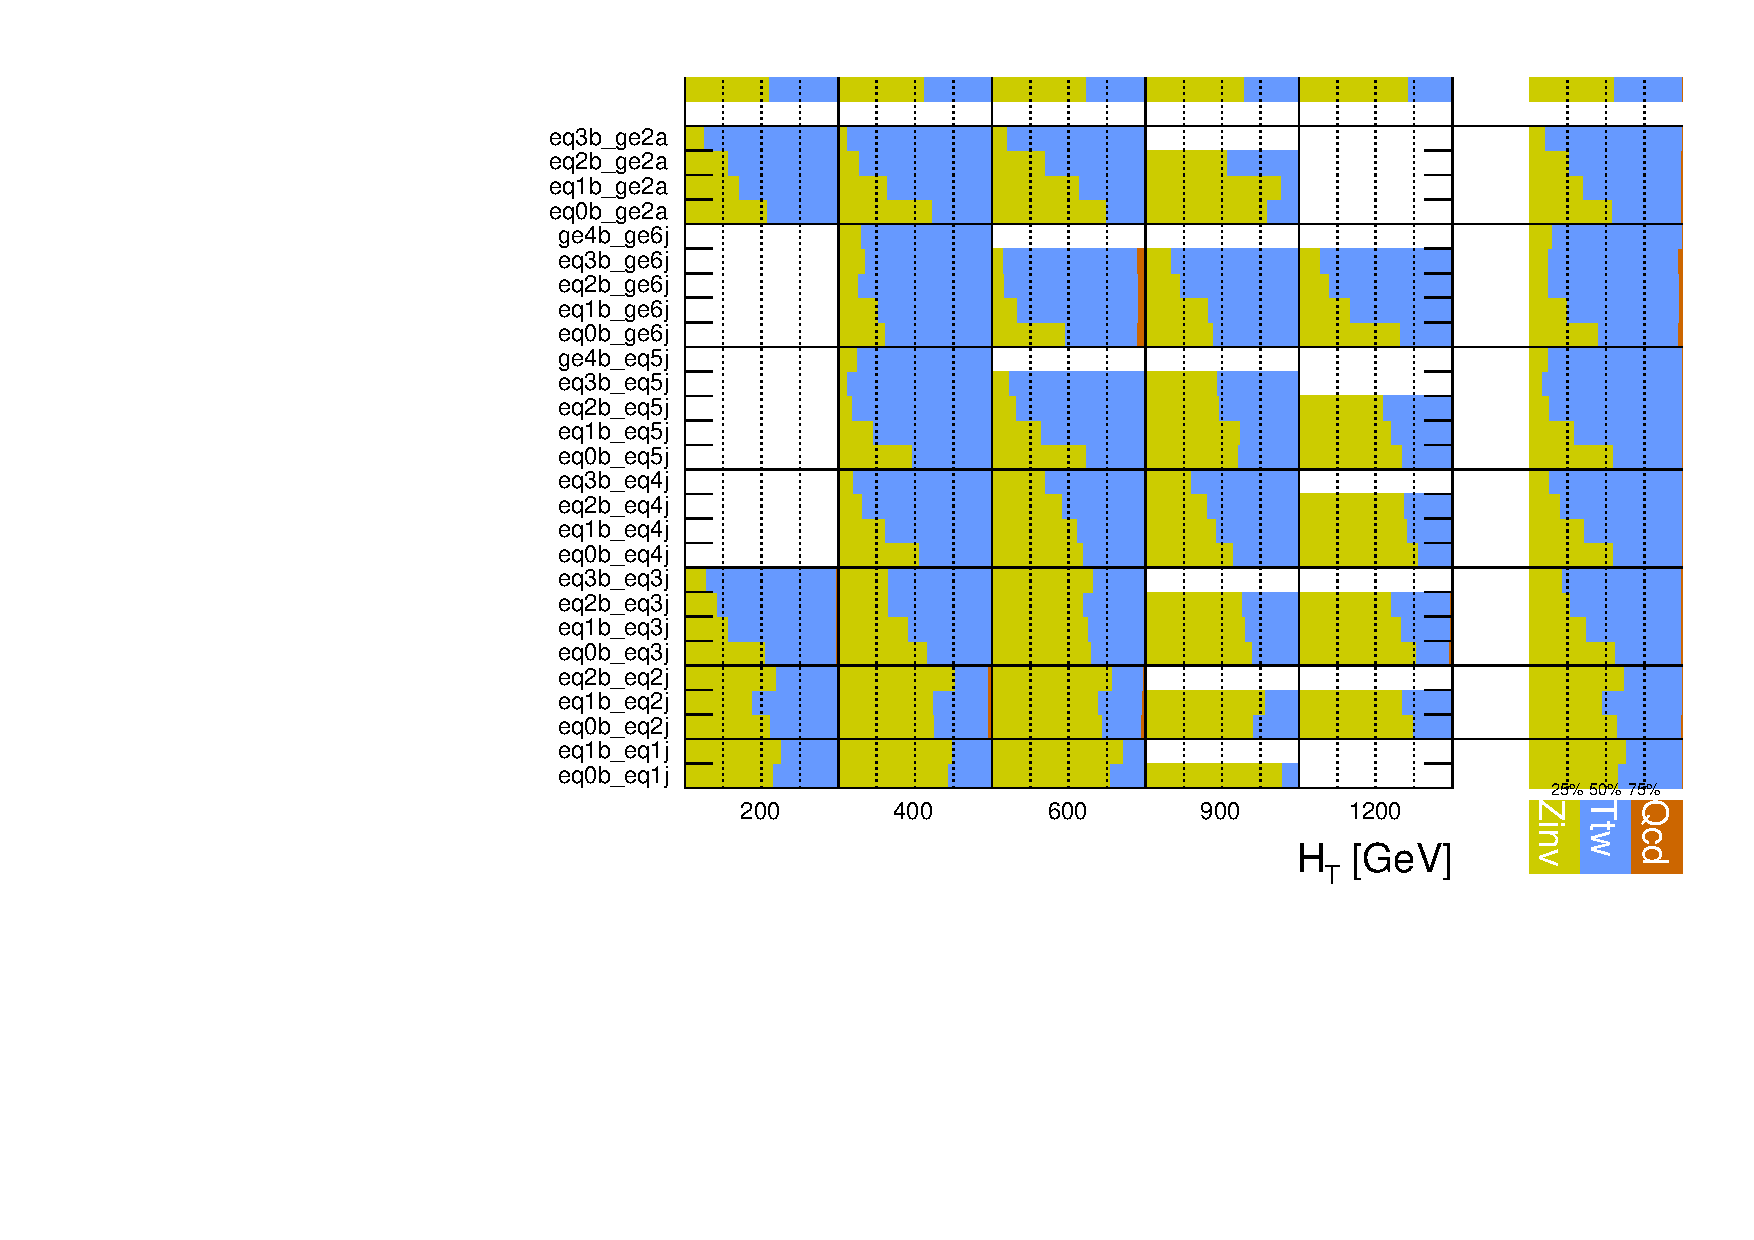
\includegraphics[width=0.6\linewidth]{figures/results/36invfb/breakdown/crfit/Signal_sample_composition.pdf}\\
  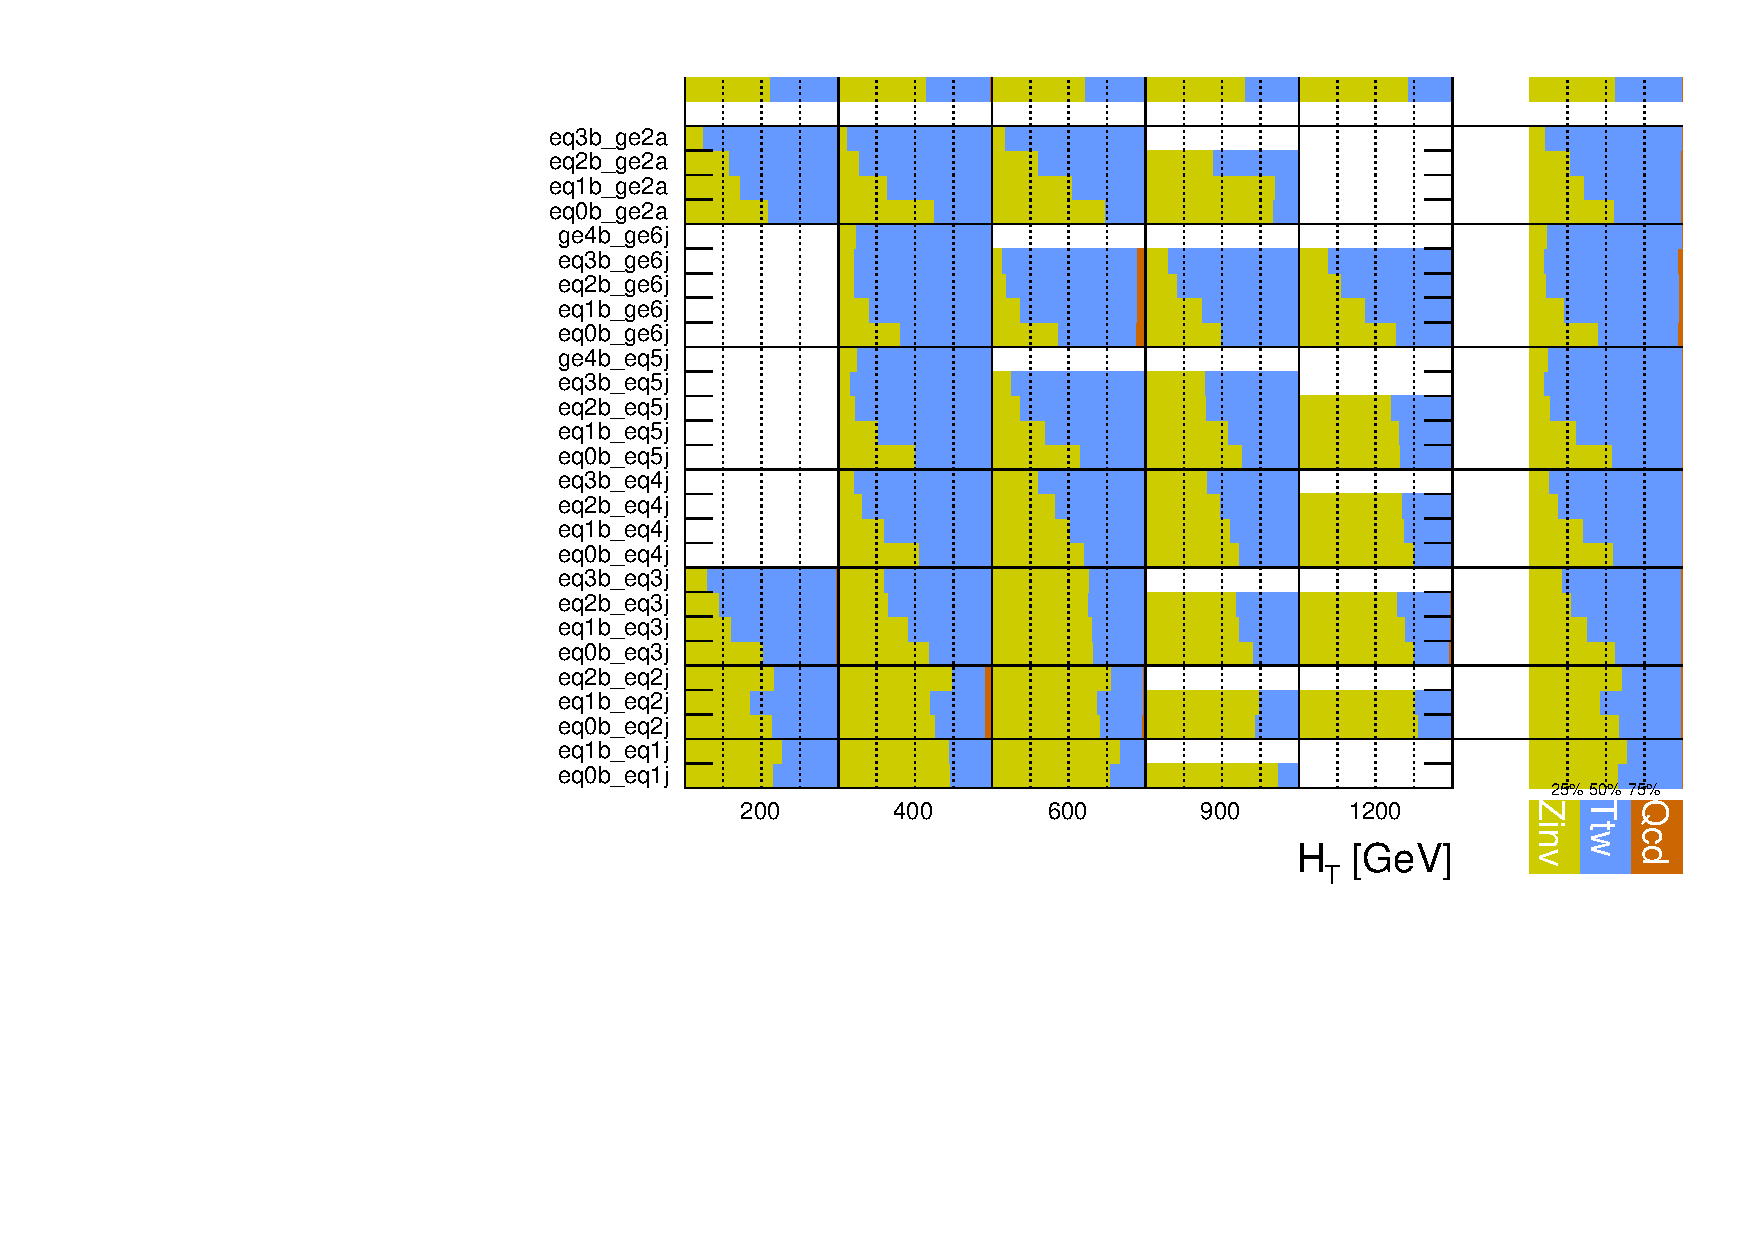
\includegraphics[width=0.6\linewidth]{figures/results/36invfb/breakdown/postfit/Signal_sample_composition.pdf}
\end{figure}

